%%%%%%%%%%%%%%%%%%%%%%%%%%%%%%%%%%%%%%%%%%%%%%%%%%%%%%%%%%%%%%%%%%%%%%
%  第 1 个逻辑月 · 月度报告
%  主题：小块：从抽象到具体（复现学长 + UDF 基线 + 算法提要）
%
%  说明：本报告由三人的既有材料按组长提纲的逻辑月重排而成。
%        尚无素材之处按规范留空并标注，不编造。
%  编译：xelatex 本文件（跑两遍）
%%%%%%%%%%%%%%%%%%%%%%%%%%%%%%%%%%%%%%%%%%%%%%%%%%%%%%%%%%%%%%%%%%%%%%
\documentclass[stage1,fontset=fandol]{ydzjreport}

% 复现云图使用 (a)(b) 子图编号，需在 caption 之后加载 subcaption
\usepackage{subcaption}

\stageonesetup
{第 1 个逻辑月 · 基础建立}%
{冯旭东、陈思文}%
{复合微通道分区冷却}%
{【待确认】逻辑月 1 对应的自然月}%
{小块划分；学长复现；水物性 UDF；算法提要}%
{确立小块的划分方式，复现学长的建模与物理性质（UDF）思路，
	并完成控制方向的算法提要。
}%

\begin{document}
	\makestageonehead
	
	% ==================================================================
	\section{本月研究任务}
	
	\subsection{任务目标}
	
	本月项目的核心任务关键词为
	\textbf{「复现已有调研论文+课题组学长提供资料的结构、了解液体换热物理性质，编写对应变物性UDF，初步搭建冷板思路，初步构建控制流程」}、
	据此分解为四项任务：
	
	\begin{enumerate}
		\item 通过阅读文献确立\textbf{冷板的优化方式}，把空间不均匀热需求落实为研究的结构；
		\item 复现已有文献、课题组学长在\textbf{结构建模}上的思路；
		\item 复现已有文献、课题组学长在\textbf{物理性质（UDF）}上的设置，并核查其正确性；
		\item 初步控制方向完成\textbf{流程框架构建}。
	\end{enumerate}
	
	\subsection{完成情况}
	
	\begin{table}[H]
		\centering
		\caption{本月任务完成情况}
		\label{tab:tasks}
		\begin{tabularx}{\textwidth}{@{}Y c Y@{}}
			\toprule
			\rowcolor{ydzjlight} 任务 & 状态 & 说明 \\
			\midrule
			小块划分方式确立 & 部分完成 & 已形成概念表述，具体结构待进一步探究 \\
			学长结构建模复现 & 已完成 & 已复现论文中的多种流道布局 \\
			学长物性（UDF）思路复现 & 已完成 & 核查后发现原函数存在误差 \\
			控制算法提要 & 已完成 & 文献要点与二阶对象特性已整理 \\
			\bottomrule
		\end{tabularx}
	\end{table}
	
	
	% ==================================================================
	\section{核心概念梳理}
	
	\subsection{概念一：非均匀热载荷与“拼图式”小块划分}
	
	芯片热流密度在空间上高度不均匀：结区集中发热，背景区几乎不发热。
	若采用均匀结构，背景区会被「一视同仁」地强力冷却，形成\textbf{过度冷却}——
	既拉大温度梯度，又浪费泵功。
	
	\textbf{“拼图式”小块}的作用，是把连续冷板上的空间不均匀热需求，转化为
	\textbf{可单独研究、可单独供液}的流道单元。
	
	需要说明的是：各小块在连续冷板上形成不同几何区域，
	\textbf{并不必然意味着把冷板机械切开或完全隔热}。
	先研究单元、再研究组合，有利于识别各形态的作用，
	并为独立供液或流量调控预留条件。
	
	\textcolor{red}{【待补：小块划分概念图示意图（王佳蔚）】}
	
	\subsection{概念二：物理性质是探究的起点}
	
	（1）冷却工质水的物性随温度变化。因此\textbf{物性核查必须放在结构比较之前}。\textcolor{red}{补充UDF的编写学习过程，补充在后面，这里不需要（陈思文、王佳蔚）}
	（2）\textbf{控制策略的物理起源：为什么必须控制，以及控制的物理基础。}
	
	\textbf{一、缘由：静态结构回答不了「热源会移动」。}
	
	既有的结构优化研究，大多建立在一个前提上：芯片的热载荷是静态的、空间分布已知的。
	但真实工况并非如此——计算任务在核心之间交替，热点强度与位置随之漂移\cite{wu,ji}。
	这带来两个直接后果：
	
	\begin{enumerate}
		\item 为某一静态热点定制的密集结构（局部加密针肋、扩缩口），
		一旦热点转移就丧失靶向性；而其局部高流阻反而会加剧整板的流量分配不均，
		陷入「结构越复杂、适应性越差」的困境。
		\item 被动结构在时间维度上没有调节自由度。参数化研究已指出，
		纯被动方案难以应对算力波动引起的随机热冲击\cite{laguna}。
	\end{enumerate}
	
	因此，控制的必要性并不来自「结构做得不够好」，而来自\textbf{热载荷自带时间维度}：
	\textbf{结构决定「能不能冷下来」，控制决定「此刻该给多少冷」}。
	这两件事是互补的，不是替代的。
	
	\textbf{二、物理基础：三个可以被控制利用的对象性质。}
	
	\begin{enumerate}
		\item \textbf{执行量到换热系数：单调但收益递减。}
		冷却液流量由泵转速与水阀开度决定；流量增大时对流换热系数随之提高，
		但提升幅度逐渐变缓，可近似写成幂律关系
		$h = h_0 (Q/q_0)^n$，其中指数 $0<n<1$。
		这决定了「加流量有效，但边际收益递减」，也说明一味加大流量并不划算。
		
		\item \textbf{热容到惯性：一阶环节。}
		把芯片—冷板—冷却液视为一个热容节点，能量守恒给出
		$C\,\mathrm{d}T/\mathrm{d}t = Q_{\mathrm{heat}} - hA\,(T - T_f)$，
		其时间常数 $\tau = C/(hA)$。
		这是被控对象的主惯性，决定了温度对流量变化的响应快慢。
		
		\item \textbf{输运与扩散到纯滞后。}
		冷却液从阀门流到芯片、热量从结区传到测点，都需要时间；
		控制输入到温度输出之间存在纯滞后。
		于是对象近似为「一阶惯性 + 纯滞后」（FOPDT）模型。
		滞后是控制设计中真正的约束：\textbf{滞后越大，可用的反馈增益越低，响应越慢，越容易振荡}。
	\end{enumerate}
	
	\textbf{三、能量学基础：控制为什么能省功。}
	
	水力功耗随流量的增长远快于换热能力：泵功近似与流量的三次方成正比
	（$P_{\mathrm{hyd}} \propto Q^3$），而换热系数只按 $Q^n$（$n<1$）增长。
	因此「全程大流量」的代价非常高；而按需供液可以在热指标不明显劣化的前提下
	大幅降低泵功。\textbf{这正是控制的价值来源——不是让温度更低，而是让温度「恰好够低」}。
	
	\textbf{四、由上述物理性质确定的学习重点。}
	
	\begin{table}[H]
		\centering
		\caption{物理性质与控制设计的对应关系}
		\label{tab:physics-control}
		\begin{tabularx}{\textwidth}{@{}Y Y@{}}
			\toprule
			\rowcolor{ydzjlight} 对象性质 & 对控制设计的含义 \\
			\midrule
			一阶惯性（时间常数 $\tau$） & 需要积分作用消除稳态误差；增益过高会引起振荡 \\
			纯滞后（FOPDT） & 需要微分作用或预测补偿；滞后越大，可用增益越低 \\
			执行器饱和（泵 $0$--$6000$ RPM、阀 $0$--$100\%$） & 必须做抗积分饱和，否则长时间饱和后积分项会积累成大幅超调 \\
			换热系数收益递减（$n<1$） & 存在「经济流量区间」，超出后加大流量只增加泵功 \\
			临界约束（结温上限） & 需要独立的安全约束层，优先于性能目标 \\
			\bottomrule
		\end{tabularx}
	\end{table}
	
	上述对应关系是本阶段最重要的认识：\textbf{控制算法不是从文献里抄参数，
	而是由对象的物理性质倒推出结构}。它同时解释了为什么后续要把预测（微分项的提前量）
	与经典反馈（稳健性）结合起来——滞后决定了纯反馈天然「慢半拍」。
	
	\textcolor{red}{【待补：初步控制框架与控制框图（王佳蔚）】}
	
	% ==================================================================
	\section{控制方向：自控基础学习}
	
	本月控制方向的任务是完成「算法提要」，其前提是把自动控制的基础补齐。
	学习按「经典理论 $\rightarrow$ PID 调节 $\rightarrow$ 数据驱动」三步推进，
	每一步都要求能回答「这条理论对应热控对象的哪个性质」。
	
	\subsection{一阶与二阶：超调从哪里来}
	
	\textbf{一阶系统} $G(s)=K/(\tau s+1)$：阶跃响应单调上升、\textbf{没有超调}，
	达到终值 63.2\% 用时 $\tau$，2\% 调节时间约 $4\tau$。
	由此得到一条判据：\textbf{若被控对象近似一阶，那么出现超调就说明还存在二阶环节或纯滞后}。
	
	\textbf{二阶系统}由自然频率 $\omega_n$ 与阻尼比 $\zeta$ 决定：
	超调量 $M_p = \exp\!\left(-\pi\zeta/\sqrt{1-\zeta^2}\right)$，
	调节时间约 $4/(\zeta\omega_n)$。
	这条式子给出一个容易被忽略的结论：\textbf{超调的本质是阻尼不足，而不是「控制器太激进」}。
	减少超调的正确手段是提高阻尼（引入微分作用）或降低增益，
	而不是简单地把比例项调小——后者只会让响应变慢，超调未必改善。
	
	\subsection{纯滞后的代价：为什么不能高增益快响应}
	
	闭环稳定性取决于特征根位置；工程上常用 Routh 判据或 Bode 稳定裕度判断。
	而热控对象有一个经典控制里最麻烦的环节——\textbf{纯滞后} $e^{-\tau_d s}$：
	它\textbf{不改变幅值，但持续消耗相位}。滞后越大，相位裕度越小，允许的增益越低。
	
	这就解释了为什么热管理控制不能照搬「高增益、快响应」的整定思路：
	流体输运与热扩散带来的滞后是可观的，增益一高就会振荡甚至失稳。
	\textbf{滞后的存在，是「纯反馈天然慢半拍」的物理根源}。
	
	\subsection{PID 三个作用及其代价}
	
	\begin{table}[H]
		\centering
		\caption{PID 三个作用的物理含义与代价}
		\label{tab:pid}
		\begin{tabularx}{\textwidth}{@{}c Y Y Y@{}}
			\toprule
			\rowcolor{ydzjlight} 作用 & 物理含义 & 带来什么 & 代价 \\
			\midrule
			P & 与当前误差成正比 & 立即响应，提高增益可加快响应 & 留下稳态误差；增益过大会振荡 \\
			I & 累积历史误差 & 消除稳态误差（提高无差度） & 引入约 $-90^\circ$ 相位滞后，易超调；长时间饱和会积分饱和 \\
			D & 对误差变化率作用 & 提供超前相位，改善阻尼、抑制超调 & 放大测量噪声；对纯滞后补偿能力有限 \\
			\bottomrule
		\end{tabularx}
	\end{table}
	
	与之配套的工程化措施也一并整理了三项：
	\begin{enumerate}
		\item \textbf{积分限幅（抗饱和）}：执行器到顶时冻结积分累加，
		否则退出饱和后积分项会积累成一次大幅超调；
		\item \textbf{微分先行}：微分只作用于测量值而不作用于设定值，
		避免设定值阶跃时产生冲击；
		\item \textbf{不完全微分}：微分项串入低通滤波，抑制噪声放大。
	\end{enumerate}
	
	\subsection{回到对象：两条整定上的判断}
	
	把上述理论对应回热控对象，可以收敛为两条在整定时最容易出错的判断：
	
	\begin{enumerate}
		\item \textbf{先看执行器余量，再谈参数。}
		若泵已到上限、阀已全开，而温度仍在上升，
		那么此时的超调与振荡\textbf{不是整定问题，而是能力问题}。
		调参数只会把问题掩盖成「响应变慢」。
		\item \textbf{滞后决定增益上限。}
		热控对象的相位裕度本就被纯滞后吃掉了一部分，
		照搬「快响应」的整定必然振荡；宁可把带宽降下来，
		换取稳定与可预测。
	\end{enumerate}
	
	对象性质与控制设计的逐条对应，已在前文表~\ref{tab:physics-control} 中给出，此处不再重复。
	
	\subsection{数据驱动方法的定位}
	
	在补齐经典部分后，进一步阅读了强化学习用于流动与传热控制的进展。
	一方面，深度强化学习在流场控制中确实展现出处理强非线性与时变工况的能力，
	闭环强制对流控制已有实验与数值验证\cite{wangy,wangyz}；
	另一方面，综述也明确指出，此类方法在可靠性、可解释性与稳定性量化上仍有明显短板\cite{vignon}。
	
	结合申报书确定的路线，本阶段的判断是：
	\textbf{用预测承担「提前量」，用 PID 承担「兜底」}。
	预测模型负责给出未来短时温度趋势，用以重构微分项；
	而经典反馈保留为约束执行层，保证即使预测失效也不会失控。
	这与「物理信息增强的智能自适应架构」的提法一致\cite{tao,brunton}。
	
	\subsection{本阶段认识}
	
	\begin{enumerate}
		\item \textbf{控制结构由对象性质倒推，不是从文献抄参数}。
		惯性、滞后、饱和、收益递减这四条，决定了必须用积分、微分、抗饱和与安全层。
		\item \textbf{超调要先分清来源}：是阻尼不足，还是执行器到顶。
		两者的处理方式完全不同——前者调参数，后者只能改结构或换执行器。
		\item \textbf{滞后是纯反馈的天花板}，这也是后续必须引入预测的物理动机；
		但预测不能替代反馈，只能作为前馈式的补充。
	\end{enumerate}
	
	% ==================================================================
	\section{阶段一：通读与摘录}
	
	\subsection{学习路径}
	
	\begin{enumerate}
		\item 先通读学长攻略（课题组已有经验）、结构类论文，梳理几何布局、进出口组织与边界条件；
		\item 复现其中的代表性流道，取得可对照的性能趋势；
		\item 转向物理性质：核查计算所用的水物性函数，确认随温度变化的正确性；
		\item 控制方向并线推进：整理控制文献要点与二阶对象的动态特性，形成算法提要。
	\end{enumerate}
	
	\subsection{关键摘录}
	
	

	\begin{table}[H]
	  \centering
	  \small
	  \renewcommand{\arraystretch}{1.12}
	  \caption{文献要点与本阶段工作}
	  \label{tab:notes}
	  \begin{tabularx}{\textwidth}{@{}>{\RaggedRight\arraybackslash}p{0.16\textwidth} Y Y@{}}
	    \toprule
	    \rowcolor{ydzjlight} 文献 & 论文要点 & 本阶段的应用 \\
	    \midrule
	    Ao 等\cite{ao} & 方形、圆形与六边形微通道的比较 & 复现三种流道，学习短流路与局部强化的组织方式 \\[3pt]
	    隋增光等\cite{ref1} & 综述数据中心吸收式器件散热、余热制冷、储能、发电与空气取水，强调低品位余热的多功能利用及系统集成。 & 补充研究背景与系统应用场景；在冷板研究之外，梳理出口水温、余热利用与节能节水之间的联系，拓展系统评价思路。 \\[3pt]
	    Xu 等\cite{ref2} & 针对双桥臂 SiC IGBT 多热源，研究双面液冷与六类导流微结构；海鸥形结构综合性能因子达 1.51，交错结构更利于芯片局部均温。 & 依据热源位置布置强化结构，将海鸥形、交错导流纳入候选矩阵；比较模块整体温度与局部热点温度，避免仅以平均温度筛选。 \\[3pt]

	    \bottomrule
	  \end{tabularx}
	\end{table}

	\begin{table}[H]
	  \centering
	  \small
	  \renewcommand{\arraystretch}{1.12}
	  \caption{文献要点与本阶段工作（续1）}
	  \label{tab:notes-cont-2}
	  \begin{tabularx}{\textwidth}{@{}>{\RaggedRight\arraybackslash}p{0.16\textwidth} Y Y@{}}
	    \toprule
	    \rowcolor{ydzjlight} 文献 & 论文要点 & 本阶段的应用 \\
	    \midrule
	    Wang 等\cite{ref5} & 将非等高双层通道、分形分叉与冲击射流结合，并采用实验验证和 NSGA-II 优化；文中报告最优无肋方案的 PEC 较参照结构提高 24.61\%。 & 拓展“层间高度差—分叉配流—局部冲击”的组合方案；先比较不同进水组织，再开展热性能与压降的双目标参数优化。 \\[3pt]
	    张乾坤等\cite{ref6} & 比较普通二级分支与三类叶脉仿生流道；完整五级分支相对普通结构压降降低超过 35\%，传热面温度降低超过 2 $\,{}^\circ\mathrm{C}$，综合强化因子大于 1.2。 & 将分支级数、分叉形式与网络完整性加入结构矩阵；比较流量分配、温度均匀性和压降，探索以配流优化实现强化与降阻。 \\[3pt]
	    Yang 等\cite{ref7} & 综述增材制造微通道散热器的材料、工艺、复杂流道及优化方法，讨论分布式歧管、多层结构、仿生网络与制造约束之间的关系。 & 建立候选结构的可制造性记录，关注最小特征尺寸、内壁粗糙度、残粉清理与密封；筛选既有热水力优势又便于加工验证的方案。 \\[3pt]
	    Hu 等\cite{ref8} & 比较三类吸液芯的异形均热板；顺序梯度网芯兼顾毛细回流与渗透性，最高测试热流密度达 200 W/cm$^2$，对应热阻为 0.047 K/W。 & 借鉴梯度分区与高低阻通路协同设计；将均热板作为复合散热的后续备选，并区分其相变传热机理与本阶段单相微通道模型。 \\[3pt]
	   
	    
	    Ansari 与 Kim\cite{ref13} & 针对非均匀热流，背景区使用矩形微通道、热点区布置圆柱针肋；以热阻、泵功、温度非均匀性和热点最大温升评价分区冷却。 & 建立背景区与热点区分开的热源边界条件；将局部针肋强化与全域强化进行对照，考察热点抑制效果及其额外泵功代价。 \\[3pt]
	    
	    Ma 等\cite{ref15} & 实验与模拟比较等周期和变周期正弦微通道；变周期结构增强扰动并改善均温性，但压降增大；在相同泵功下，平均热阻降低约 13\%。 & 将周期沿程变化加入几何参数矩阵；同时开展相同流量与相同泵功比较，分析下游强化能否补偿冷却液温升带来的散热衰减。 \\[3pt]
	    
	    王雅博等\cite{ref16} & 比较两端进出水与中心垂直射流配合一、二、四出口的布局；中心射流四出口方案虽非 Nu 最高，但流阻较小、综合性能更优且可避免局部热点。 & 将进口位置与出口数量作为独立变量；固定内部结构比较不同配流方式，联合考察速度死区、温度均匀性、Nu 和压降。 \\[3pt]
	    
	    Choi 等\cite{ref17} & 通过实验与 58 组数值算例研究大面积风冷 N 型歧管微通道；分析通道宽、长、高对流量分配、热阻与压降的影响，突出短流路和一体化结构的作用。 & 借鉴 N 型歧管分流与短流路设计，补充通道尺寸对配流的敏感性分析；应用于液冷时重新计算工质相关结果，保留其拓扑设计思路。 \\[3pt]
	    \bottomrule
	  \end{tabularx}
	\end{table}



	\begin{table}[H]
	  \centering
	  \small
	  \renewcommand{\arraystretch}{1.12}
	  \caption{文献要点与本阶段工作（续2）}
	  \label{tab:notes-cont-5}
	  \begin{tabularx}{\textwidth}{@{}>{\RaggedRight\arraybackslash}p{0.16\textwidth} Y Y@{}}
	    \toprule
	    \rowcolor{ydzjlight} 文献 & 论文要点 & 本阶段的应用 \\
	    \midrule
	    Indhe 等\cite{ref20} & 综述 CFD、分子动力学和人工智能在微电子散热中的应用，讨论微通道、纳米增强相变材料及复合冷却的多尺度分析与优化方法。 & 形成“参数化建模—CFD 数据积累—代理模型—优化验证”的后续路线；本阶段优先统一算例与数据字段，为机器学习准备可追溯样本。 \\[3pt]
	    Nie 等\cite{ref21} & 通过针肋关联导流结构削弱尾部流动死区并促进混合，但存在明显压降代价；在 0.15—0.8 mW 相同泵功范围内，最优结构热阻较传统针肋降低 20.8\%—22.2\%。 & 在针肋后方引入导流构件，考察高度、直径及相对偏移；结合速度场辨识强化机理，并以相同泵功对照判断额外阻力是否值得。 \\[3pt]
	    Yin 等\cite{yin} & 提出同轴开口环形 TSV 针肋，比较直列、错列与传统圆柱 TSV；综合分析 Nu、最高温度、压降、PEC、循环热应力及信号完整性。 & 借鉴开口环形针肋与错列组织方式；统一提取平均 Nu、最高温度、压降和 PEC，并将热应力作为封装可靠性的后续扩展指标。 \\[3pt]
	    Seong 等\cite{seong} & 研究倾斜肋—针肋的直列、错列及倾角效应；Re=450、倾角 60$^\circ$、热流密度 100 W/cm$^2$ 时，PEC 为 1.52，并建立 ANN 性能预测模型。 & 建立“排列方式$\times$倾角$\times$Re”参数矩阵，分析层间混合与停滞区变化；积累 CFD 数据后训练代理模型，并用独立算例验证预测结果。 \\[3pt]
	    Lorenzini 等\cite{ref24} & 在 200 $\mu$m 硅微间隙中按热点分布局部加密针肋；背景热流密度 250 W/cm$^2$、热点 250—750 W/cm$^2$、入口水温 21.3 $\,{}^\circ\mathrm{C}$ 时，所研究器件最高温度低于 65 $\,{}^\circ\mathrm{C}$。 & 建立均匀针肋与热点局部加密的对照模型；针对不同热点位置和强度匹配针肋密度，并核查旁路流动是否削弱热点区冷却。 \\[3pt]
	   
	    \bottomrule
	  \end{tabularx}
	\end{table}



	% ==================================================================
	\section{阶段二：导出与复现}
	
	\subsection{复现目标}
	
	本月复现两项内容：
	\textbf{(1)} 学长论文中的方形、圆形与六边形三种微通道的结构与流动换热组织；
	\textbf{(2)} 计算所用的水物性函数（UDF），核查其随温度变化的正确性。
	
	\subsection{复现环境与步骤}
	
	\textbf{环境}：ANSYS Fluent，工质为水，固体域与流体域耦合求解；
	物性核查采用 Python 后处理。
	
	\textbf{步骤}：
	
	\begin{enumerate}
		\item 按论文的方形、圆形与六边形布局分别构造流道，梳理流体域、固体域与加热区域；
		\item 对照论文的边界条件与求解方法开展计算，检查残差与监测量；
		\item 对三种结构做趋势对照，关注热负荷与流量变化下的温度响应；
		\item 核查原水物性 UDF：在 298.15 K 校验点比对参考物性值；
		\item 记录误差量级，判断是否需要重新拟合。
	\end{enumerate}

	
	\begin{figure}[H]
		\centering
		\begin{subfigure}{0.235\textwidth}
			\centering
			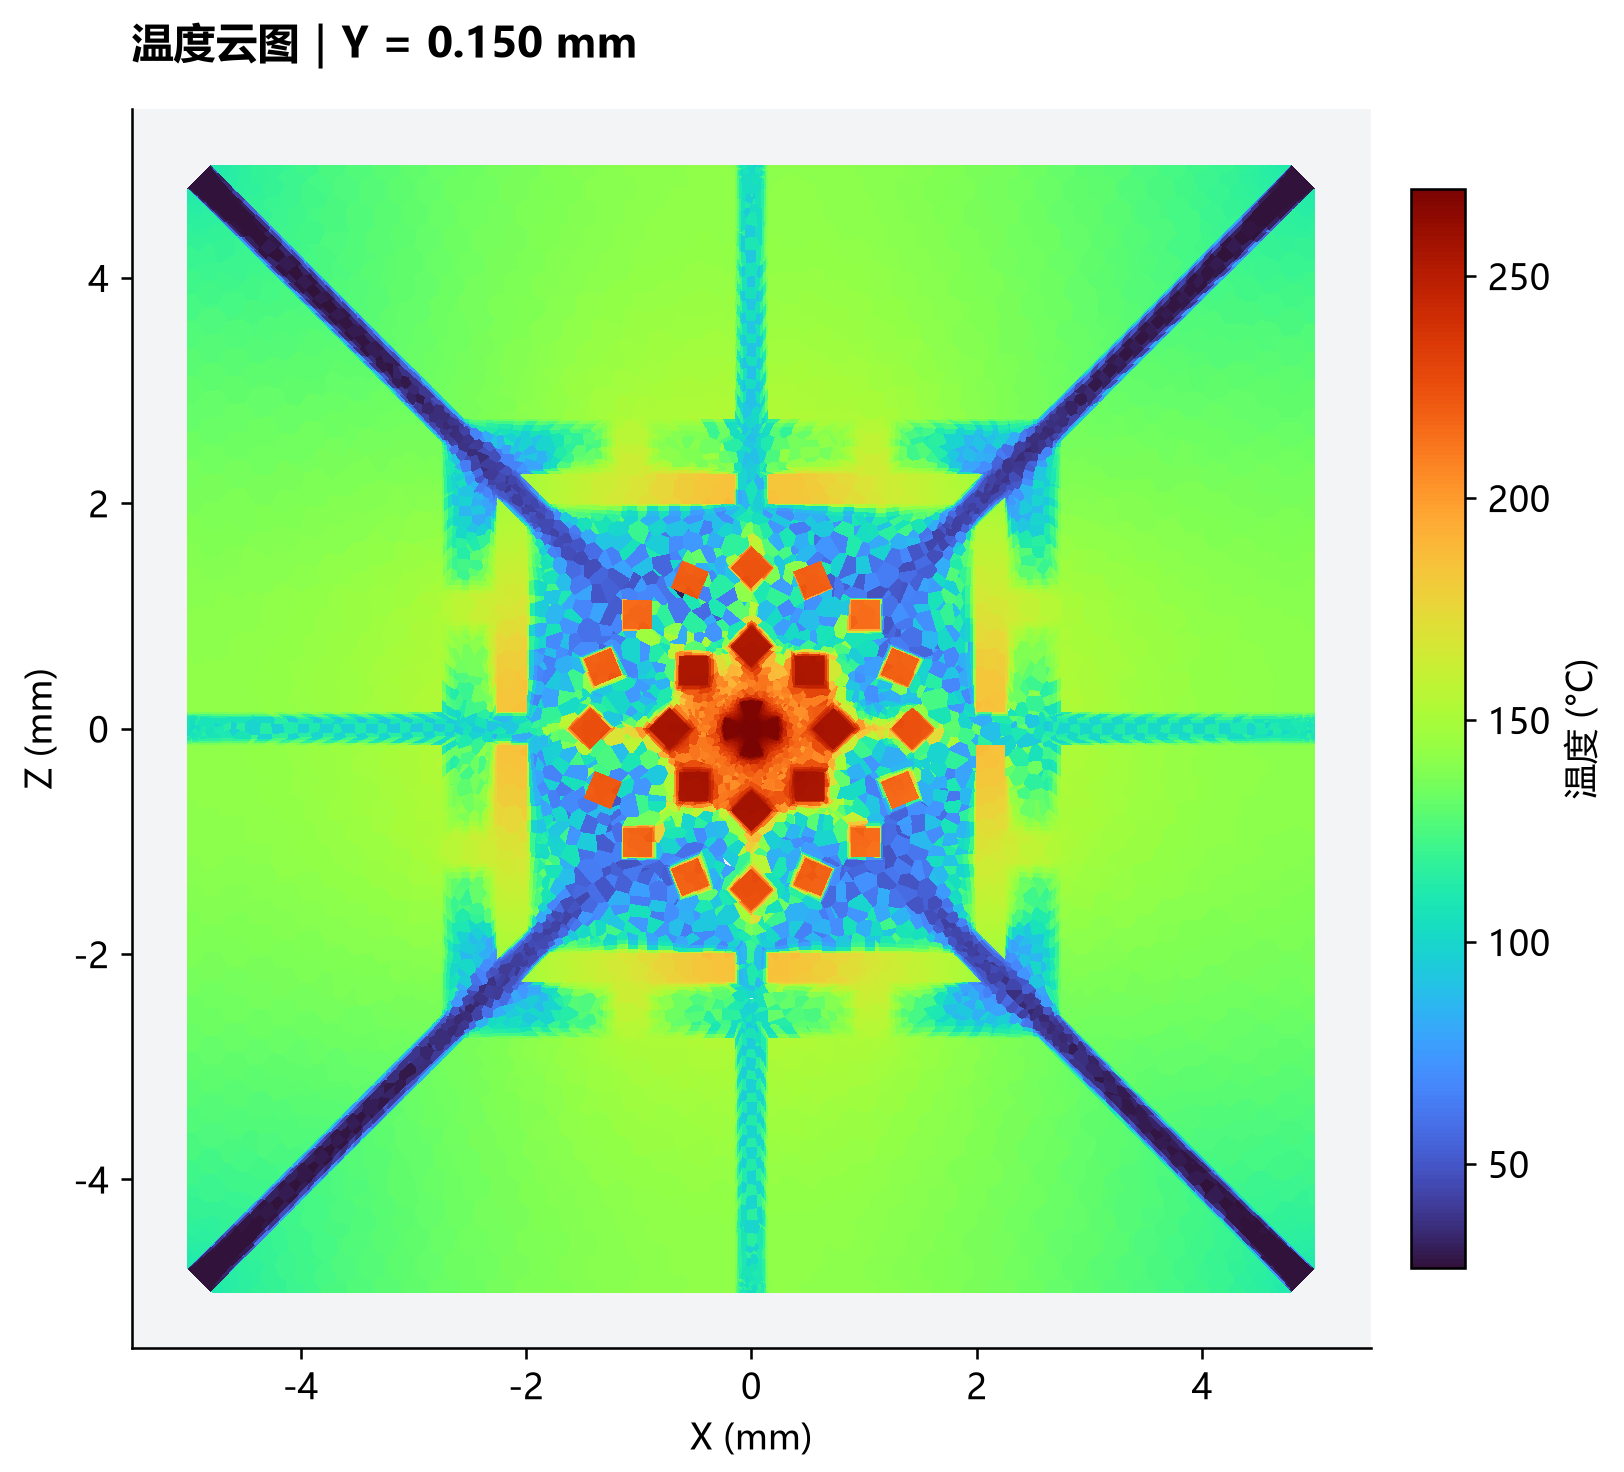
\includegraphics[width=\linewidth]{figs/01_temperature_midplane.png}
			\caption{方形微通道温度}
			\label{fig:repro-t}
		\end{subfigure}\hfill
		\begin{subfigure}{0.235\textwidth}
			\centering
			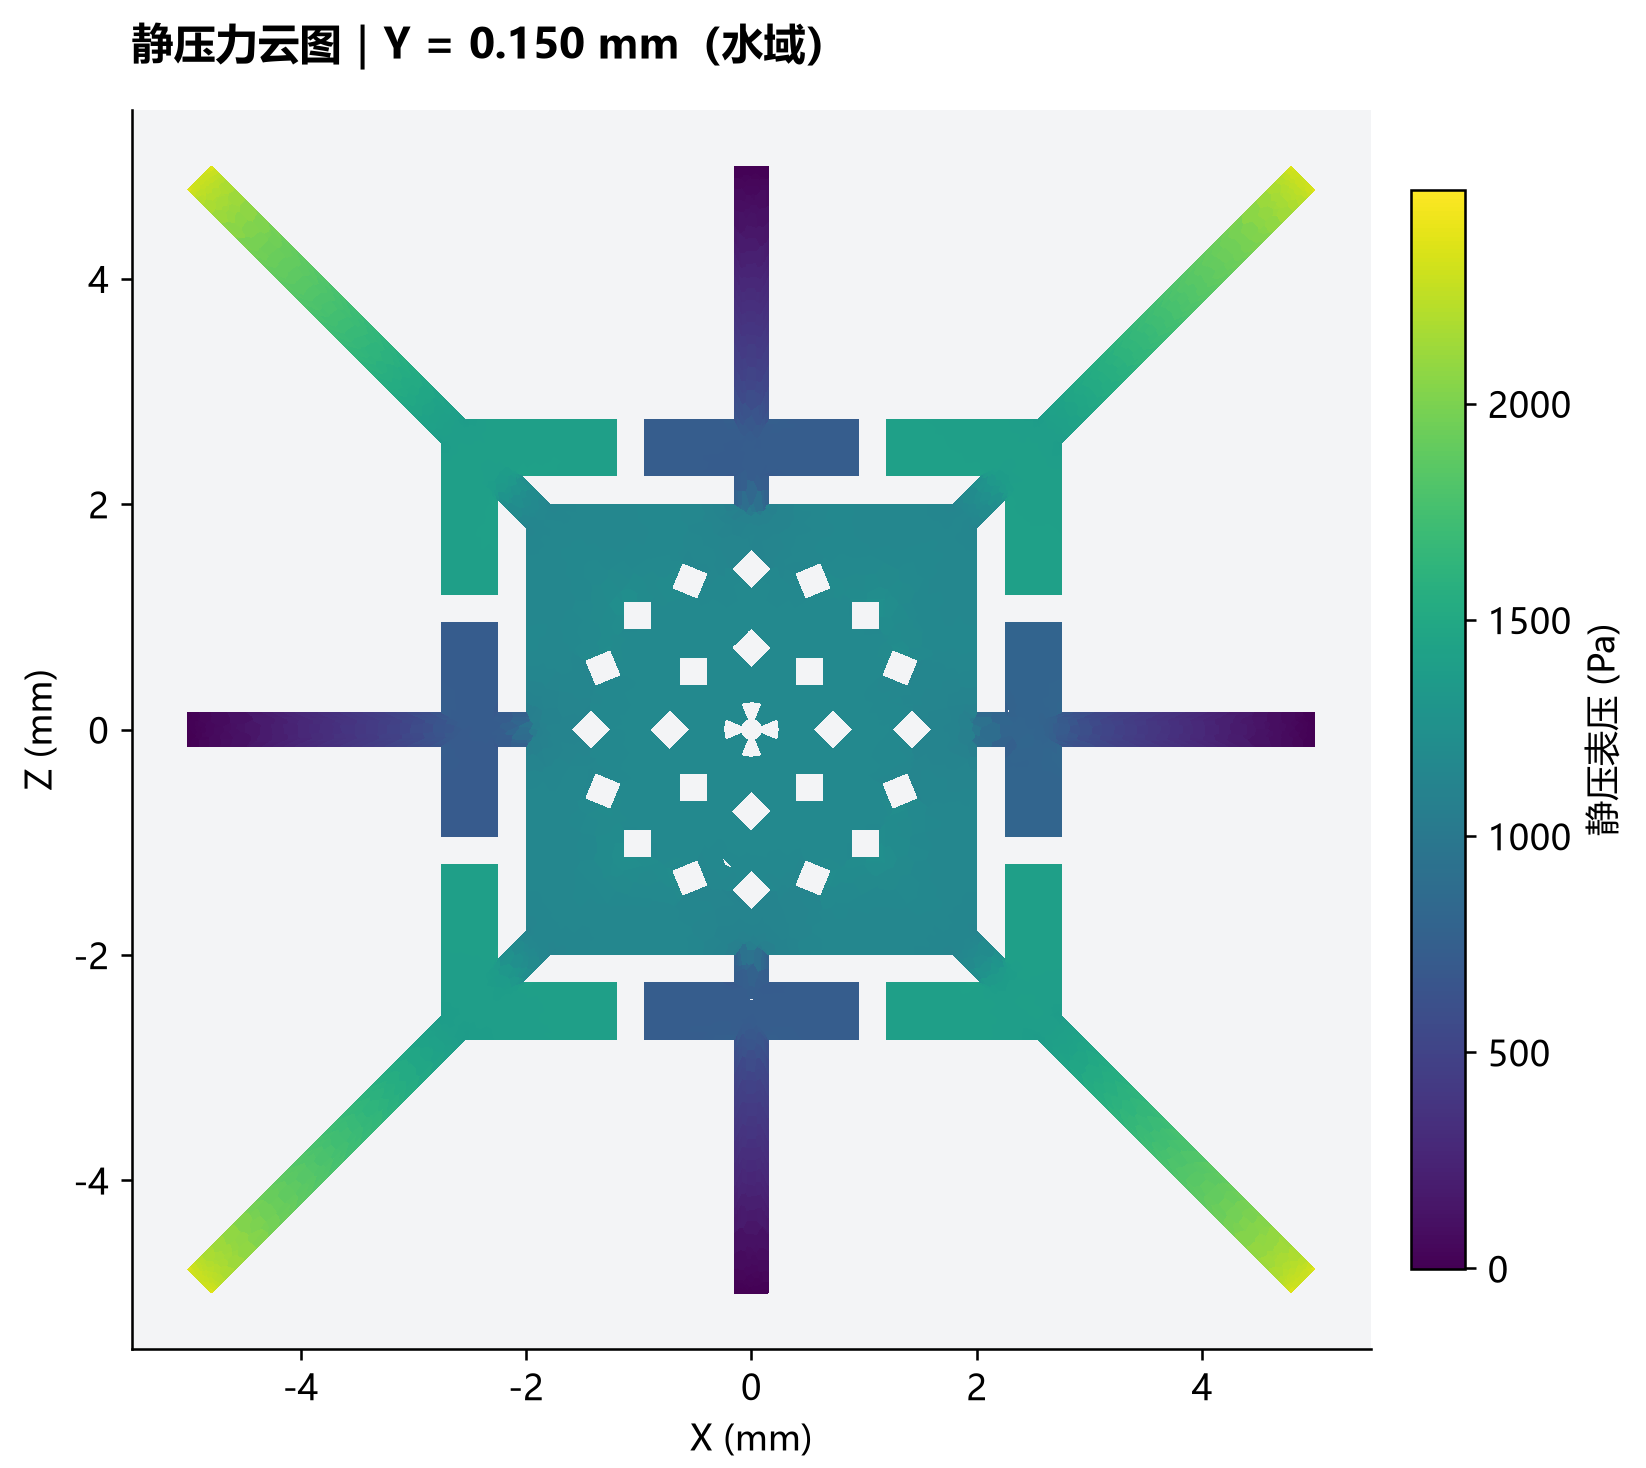
\includegraphics[width=\linewidth]{figs/02_pressure_midplane.png}
			\caption{方形微通道静压}
			\label{fig:repro-p}
		\end{subfigure}\hfill
		\begin{subfigure}{0.235\textwidth}
			\centering
			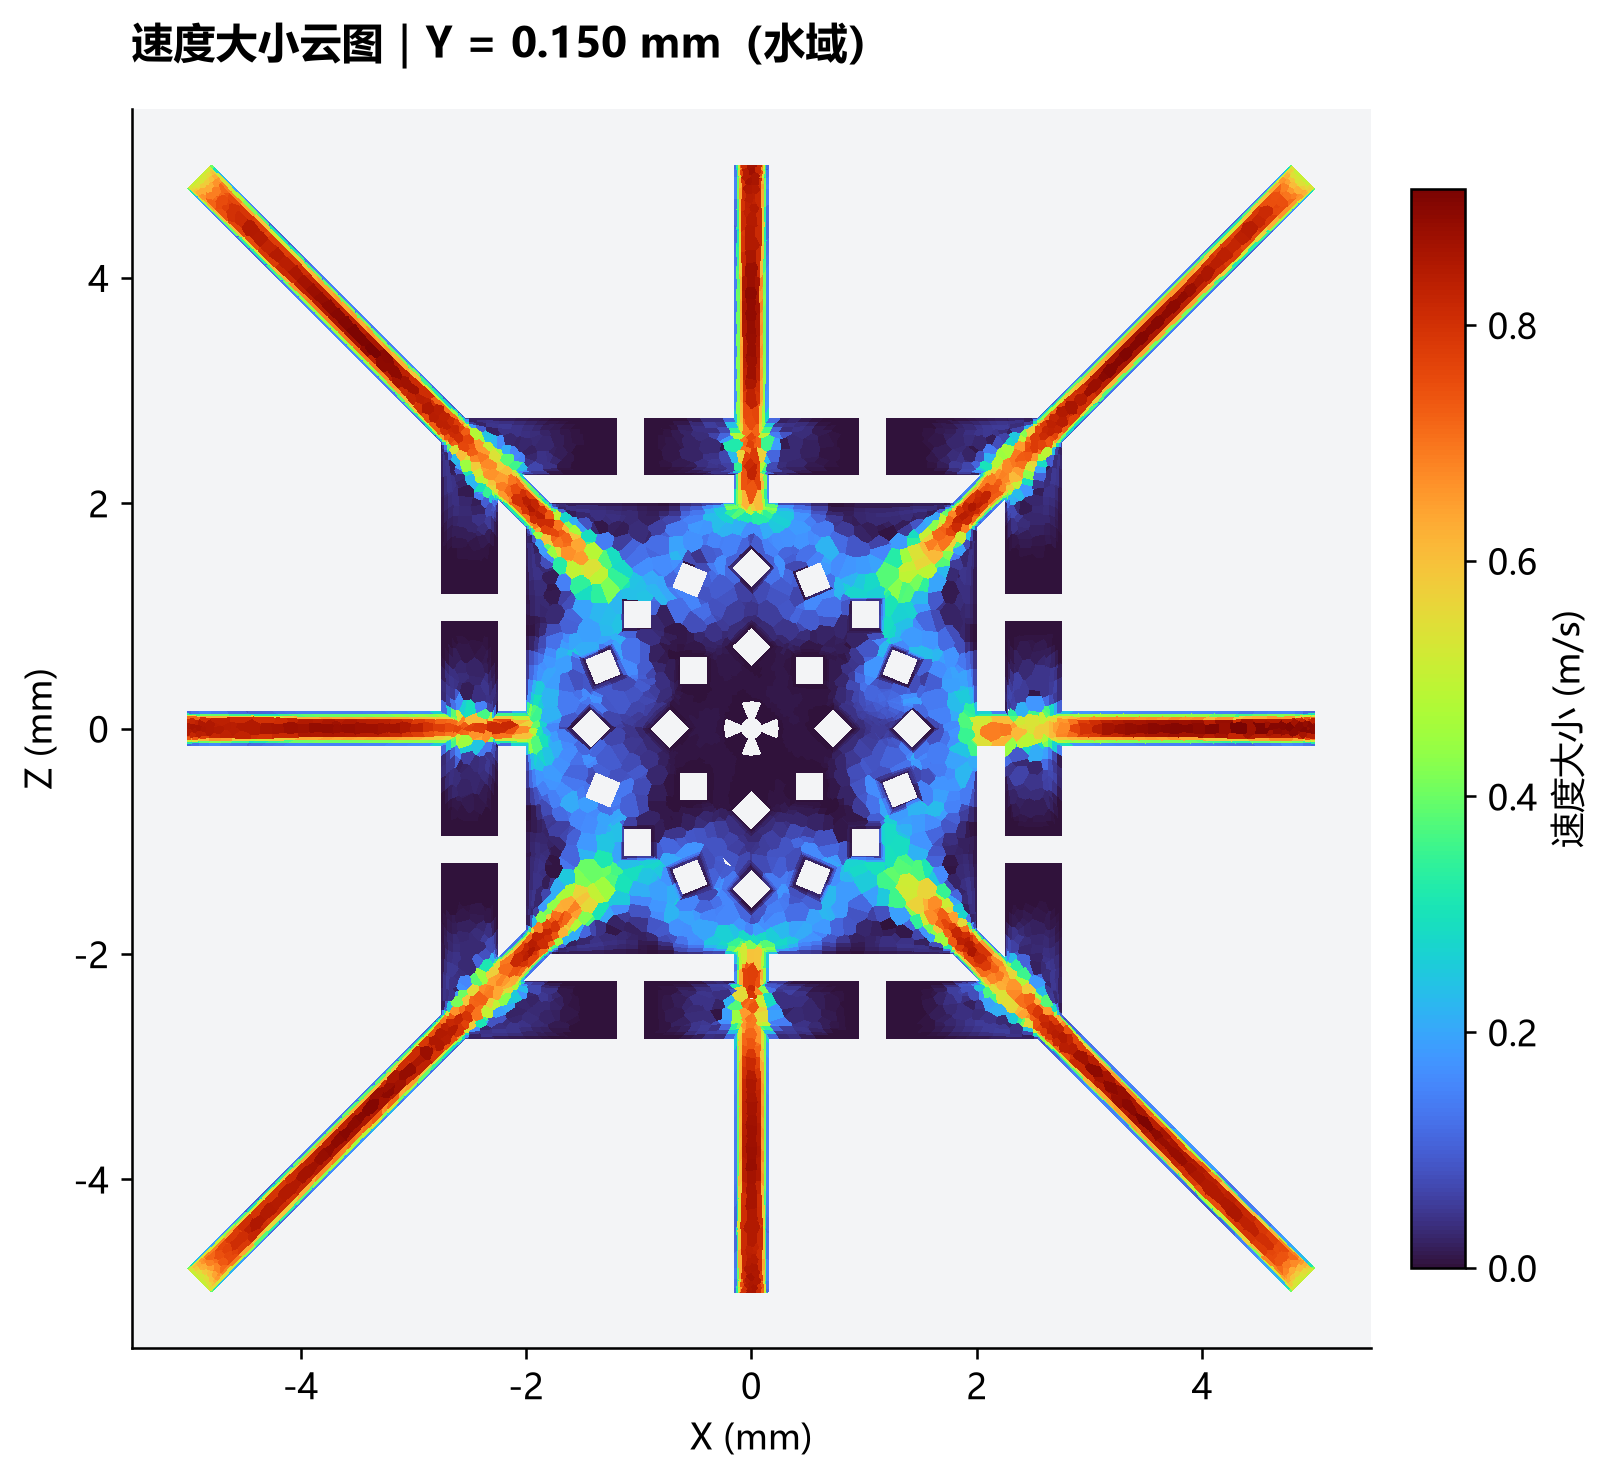
\includegraphics[width=\linewidth]{figs/03_speed_midplane.png}
			\caption{方形微通道速度大小}
			\label{fig:repro-v}
		\end{subfigure}\hfill
		\begin{subfigure}{0.235\textwidth}
			\centering
			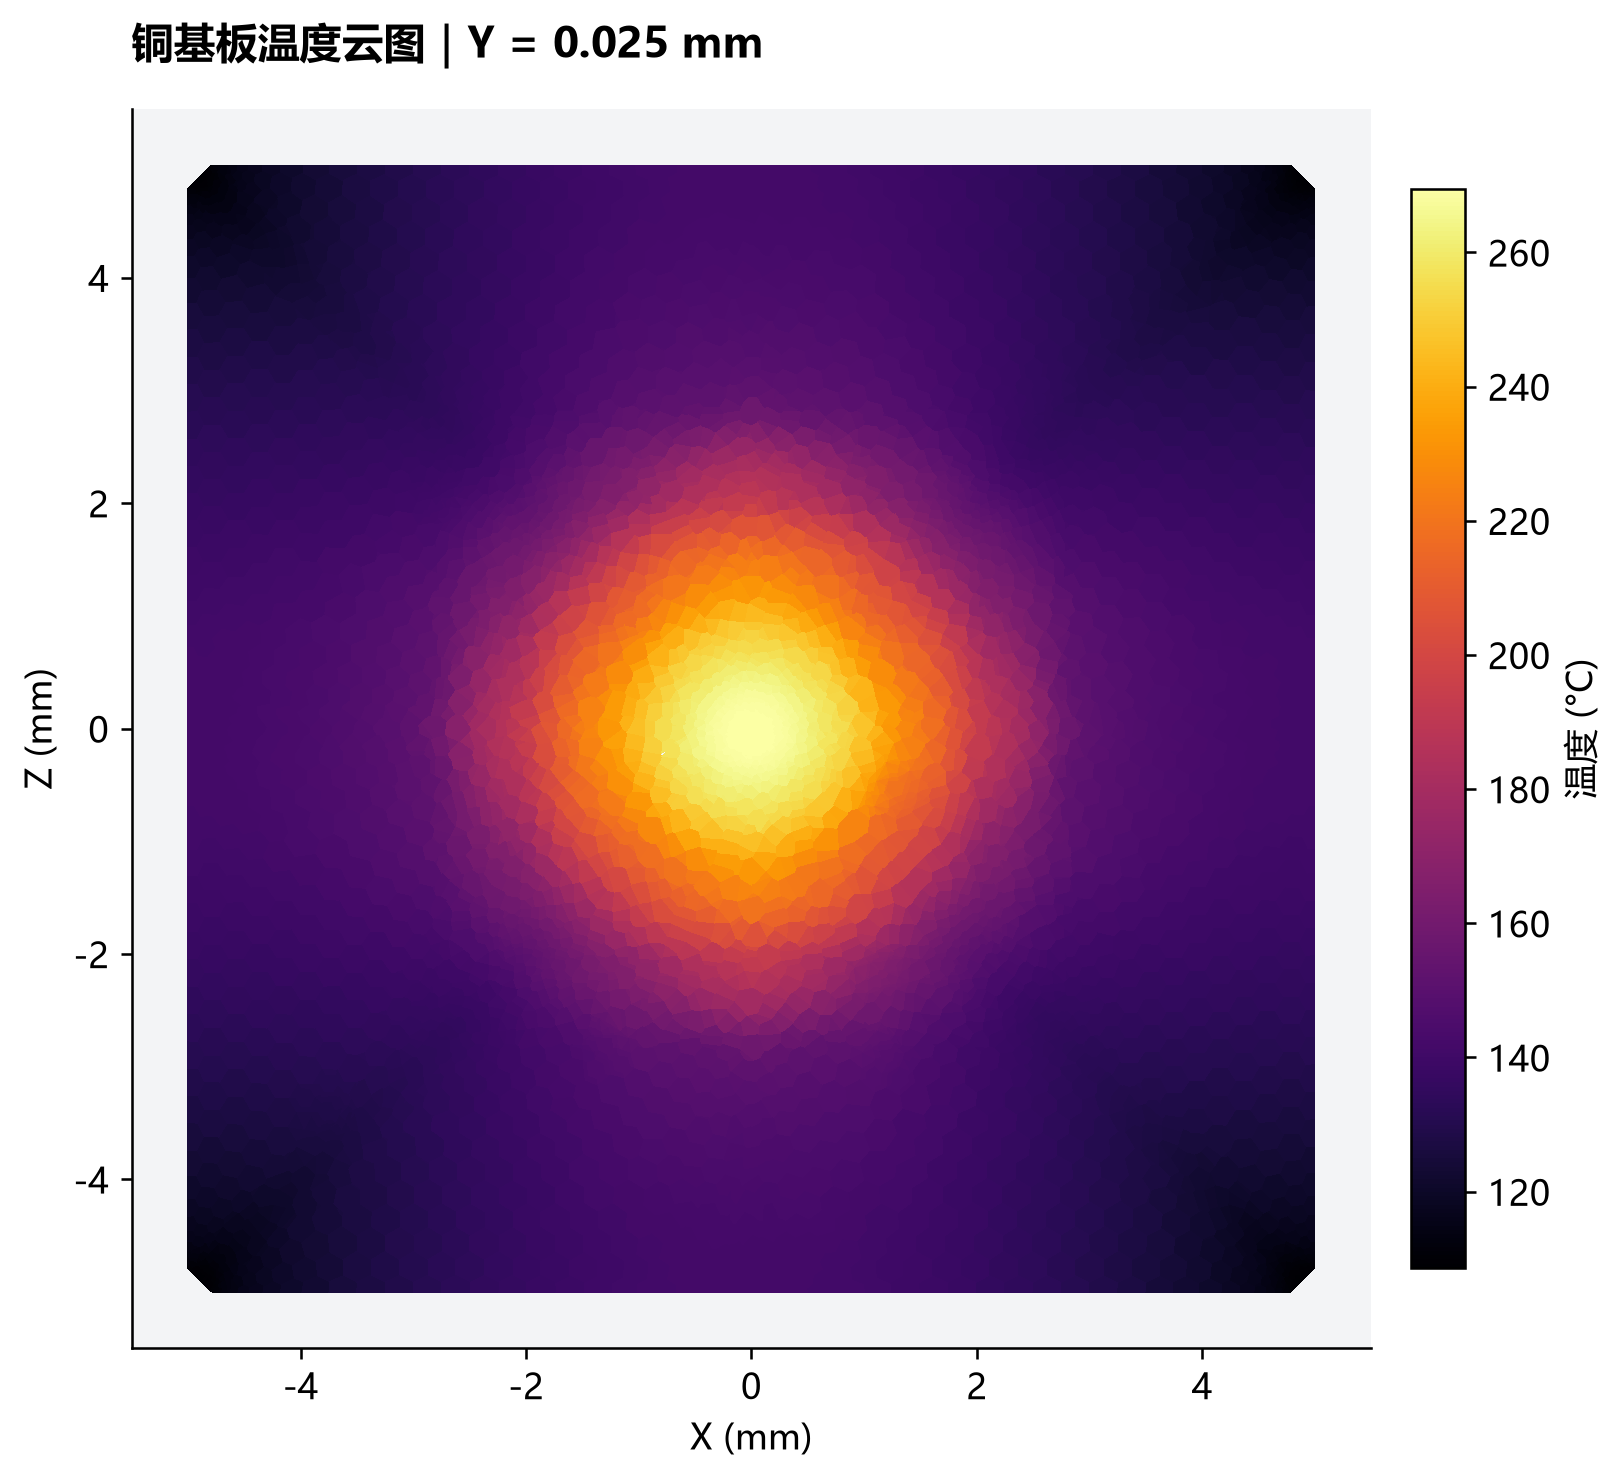
\includegraphics[width=\linewidth]{figs/04_copper_base_temperature.png}
			\caption{方形微通道铜板温度}
			\label{fig:repro-cu}
		\end{subfigure}
		
		\vspace{4pt}
		
		\begin{subfigure}{0.235\textwidth}
			\centering
			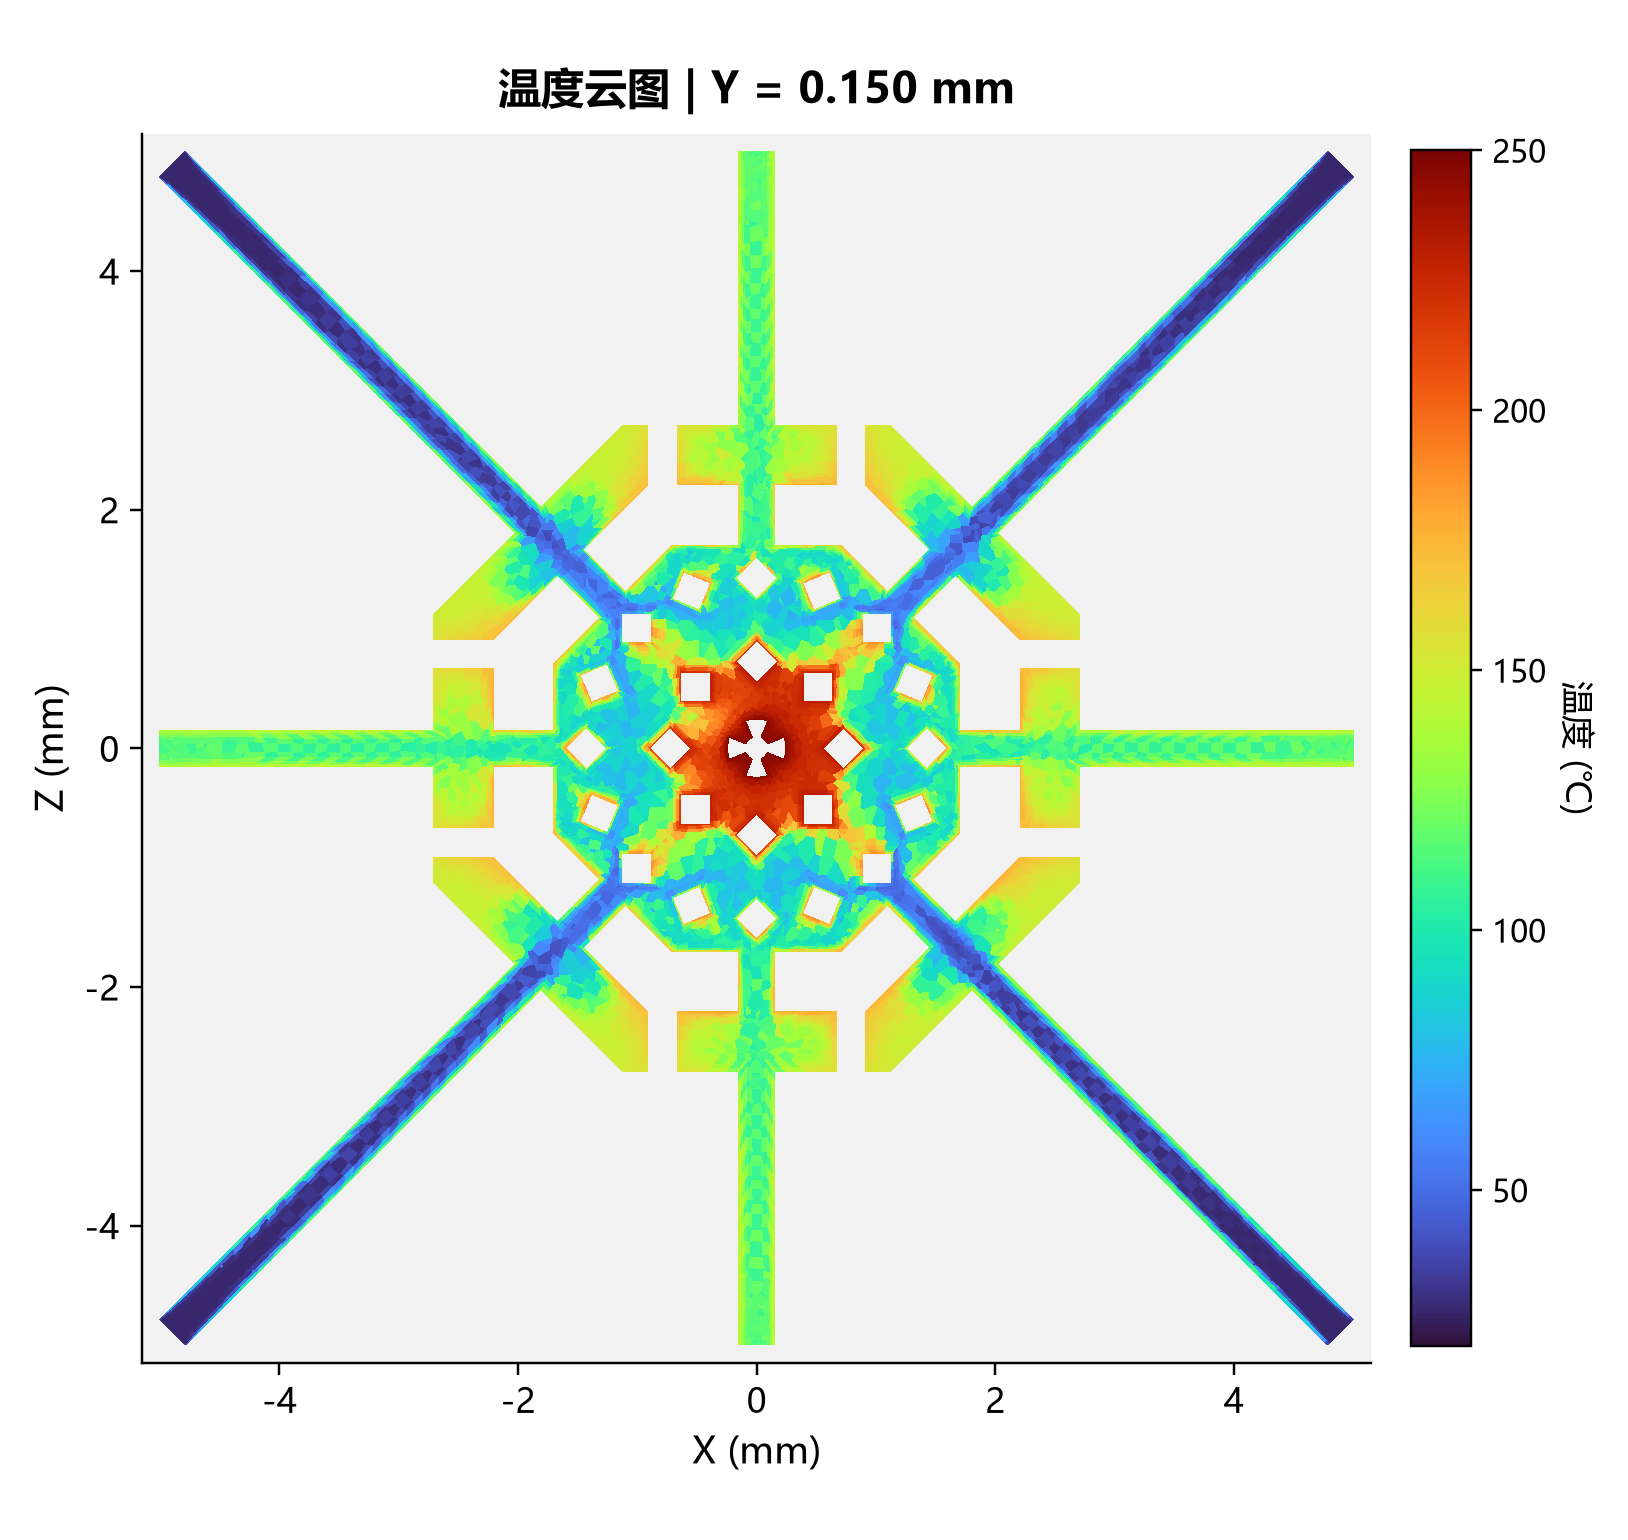
\includegraphics[width=\linewidth]{figs/05_temperature_midplane.png}
			\caption{六边形微通道温度}
			\label{fig:h5-t}
		\end{subfigure}\hfill
		\begin{subfigure}{0.235\textwidth}
			\centering
			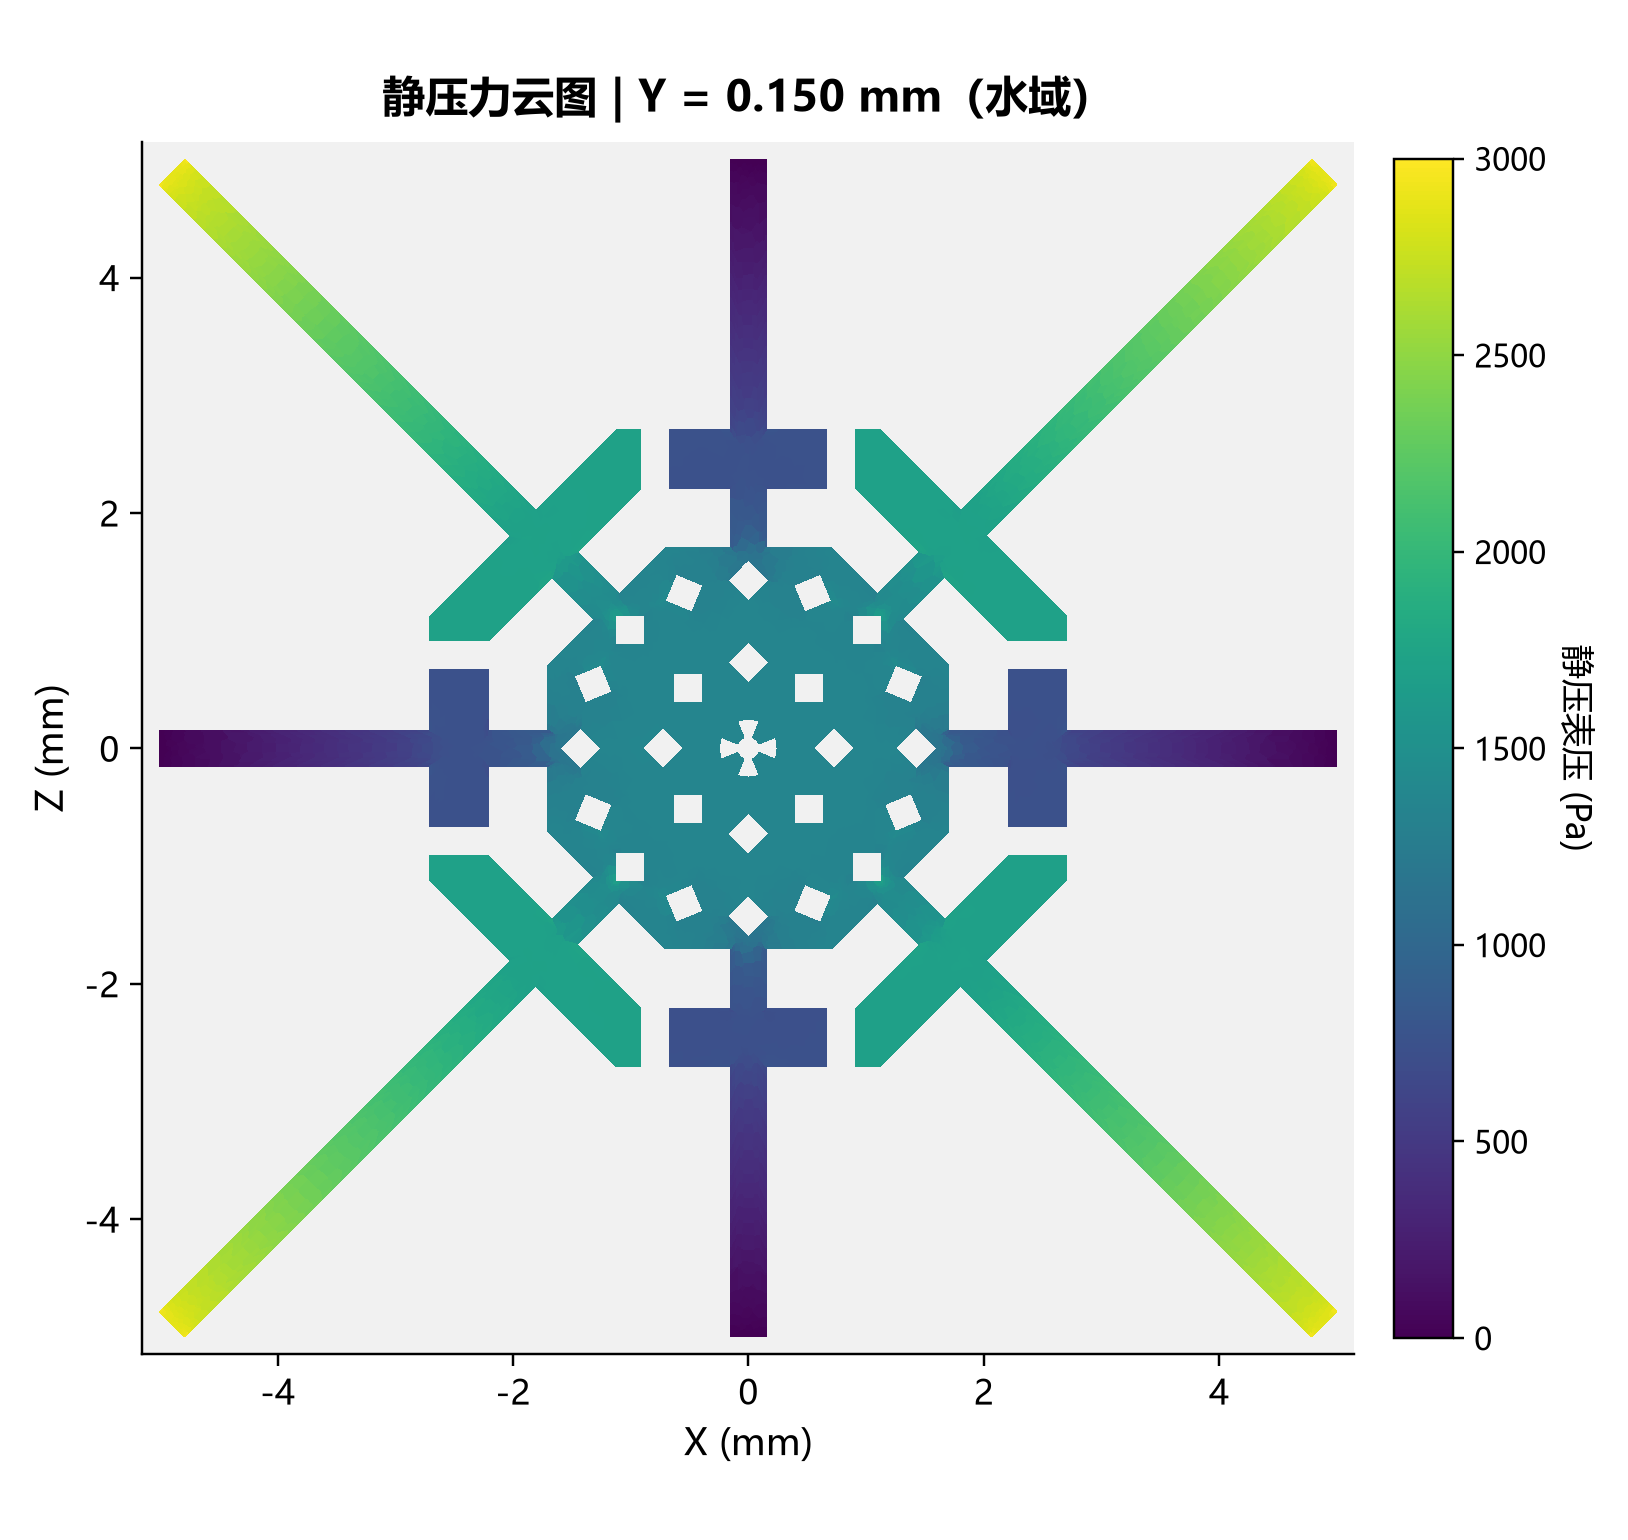
\includegraphics[width=\linewidth]{figs/06_pressure_midplane.png}
			\caption{六边形微通道静压}
			\label{fig:h5-p}
		\end{subfigure}\hfill
		\begin{subfigure}{0.235\textwidth}
			\centering
			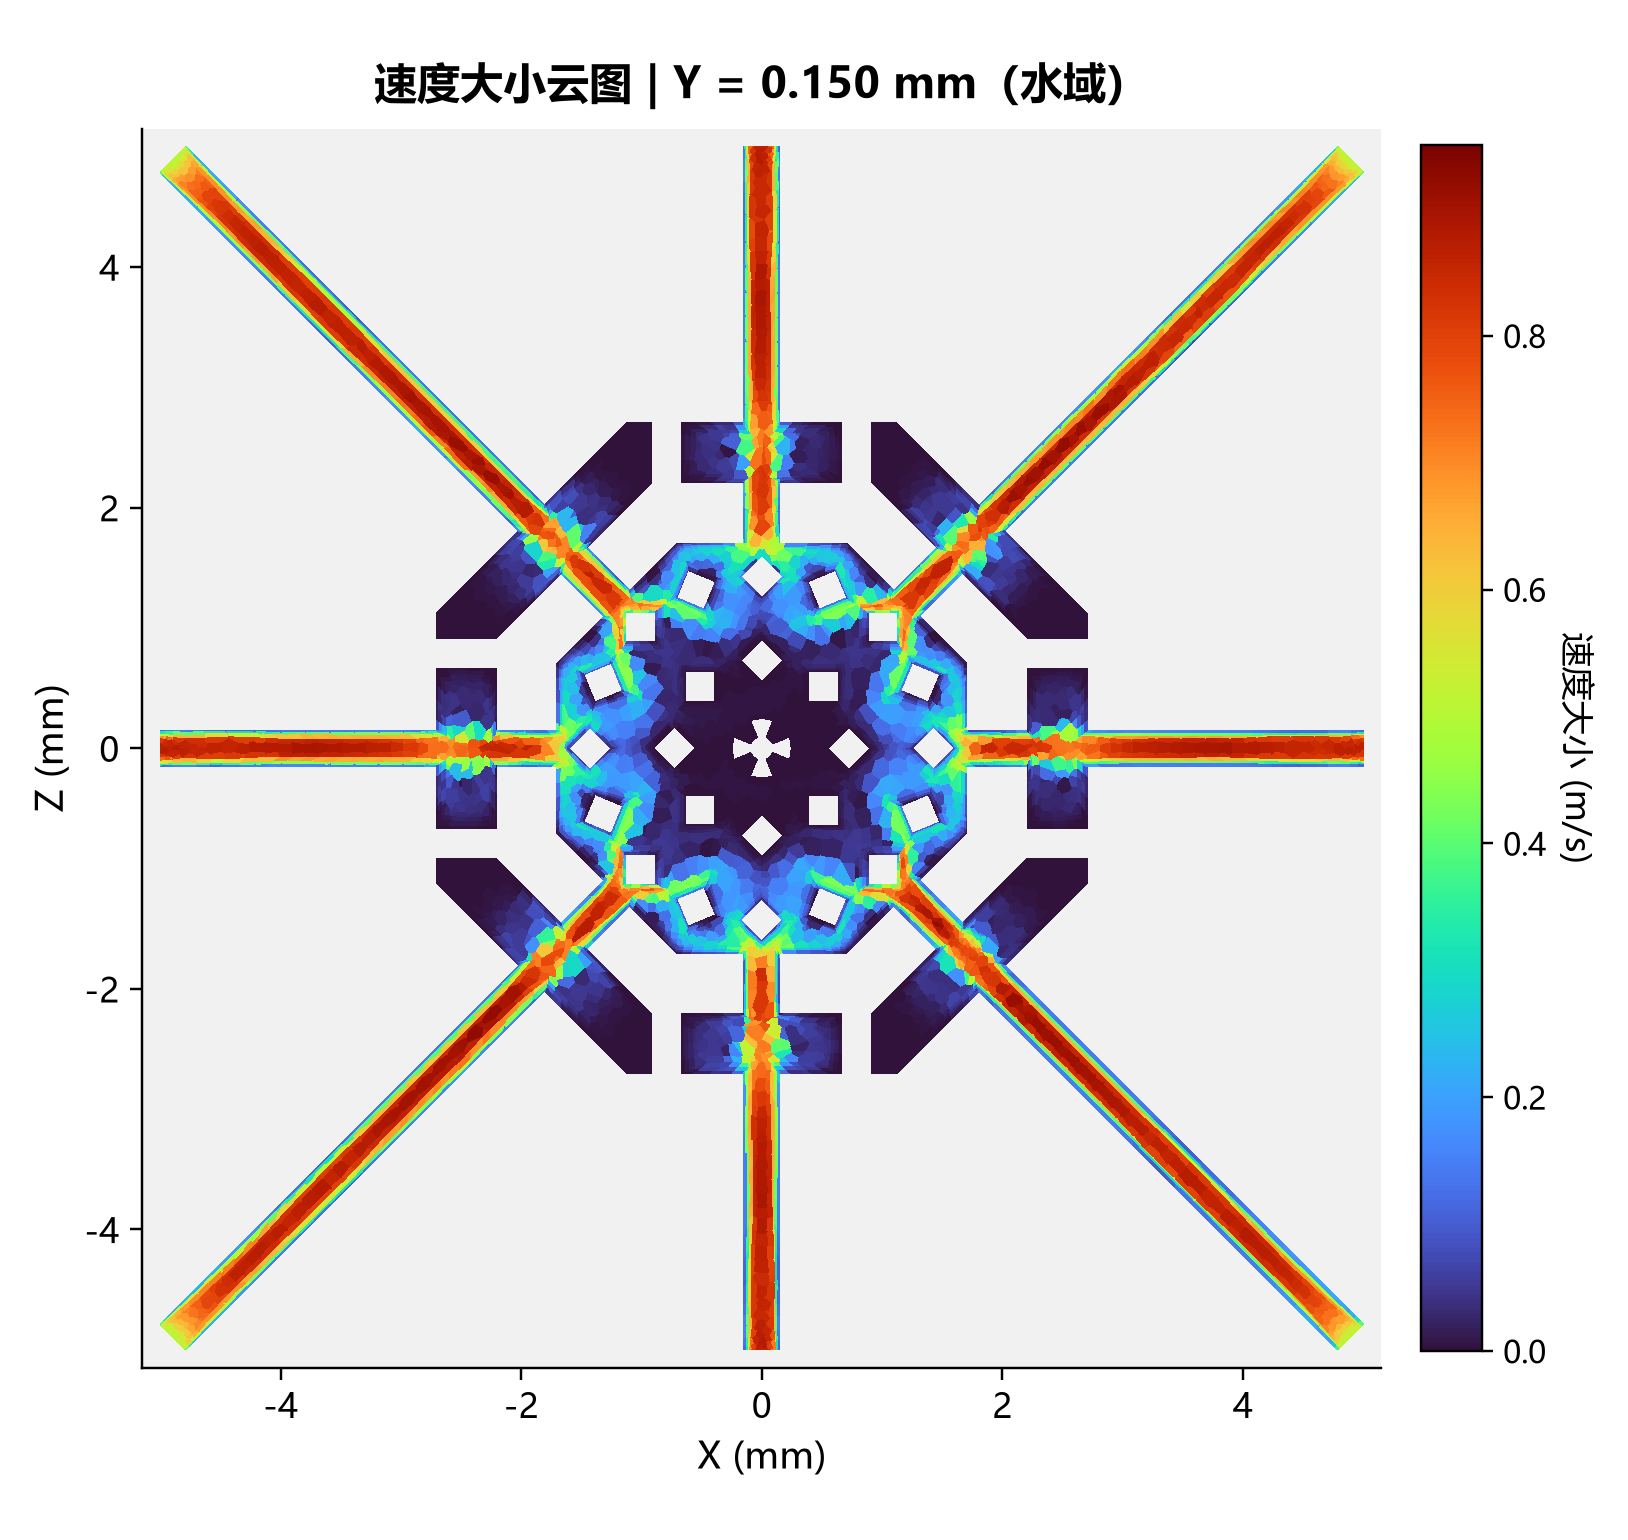
\includegraphics[width=\linewidth]{figs/07_speed_midplane.png}
			\caption{六边形微通道速度大小}
			\label{fig:h5-v}
		\end{subfigure}\hfill
		\begin{subfigure}{0.235\textwidth}
			\centering
			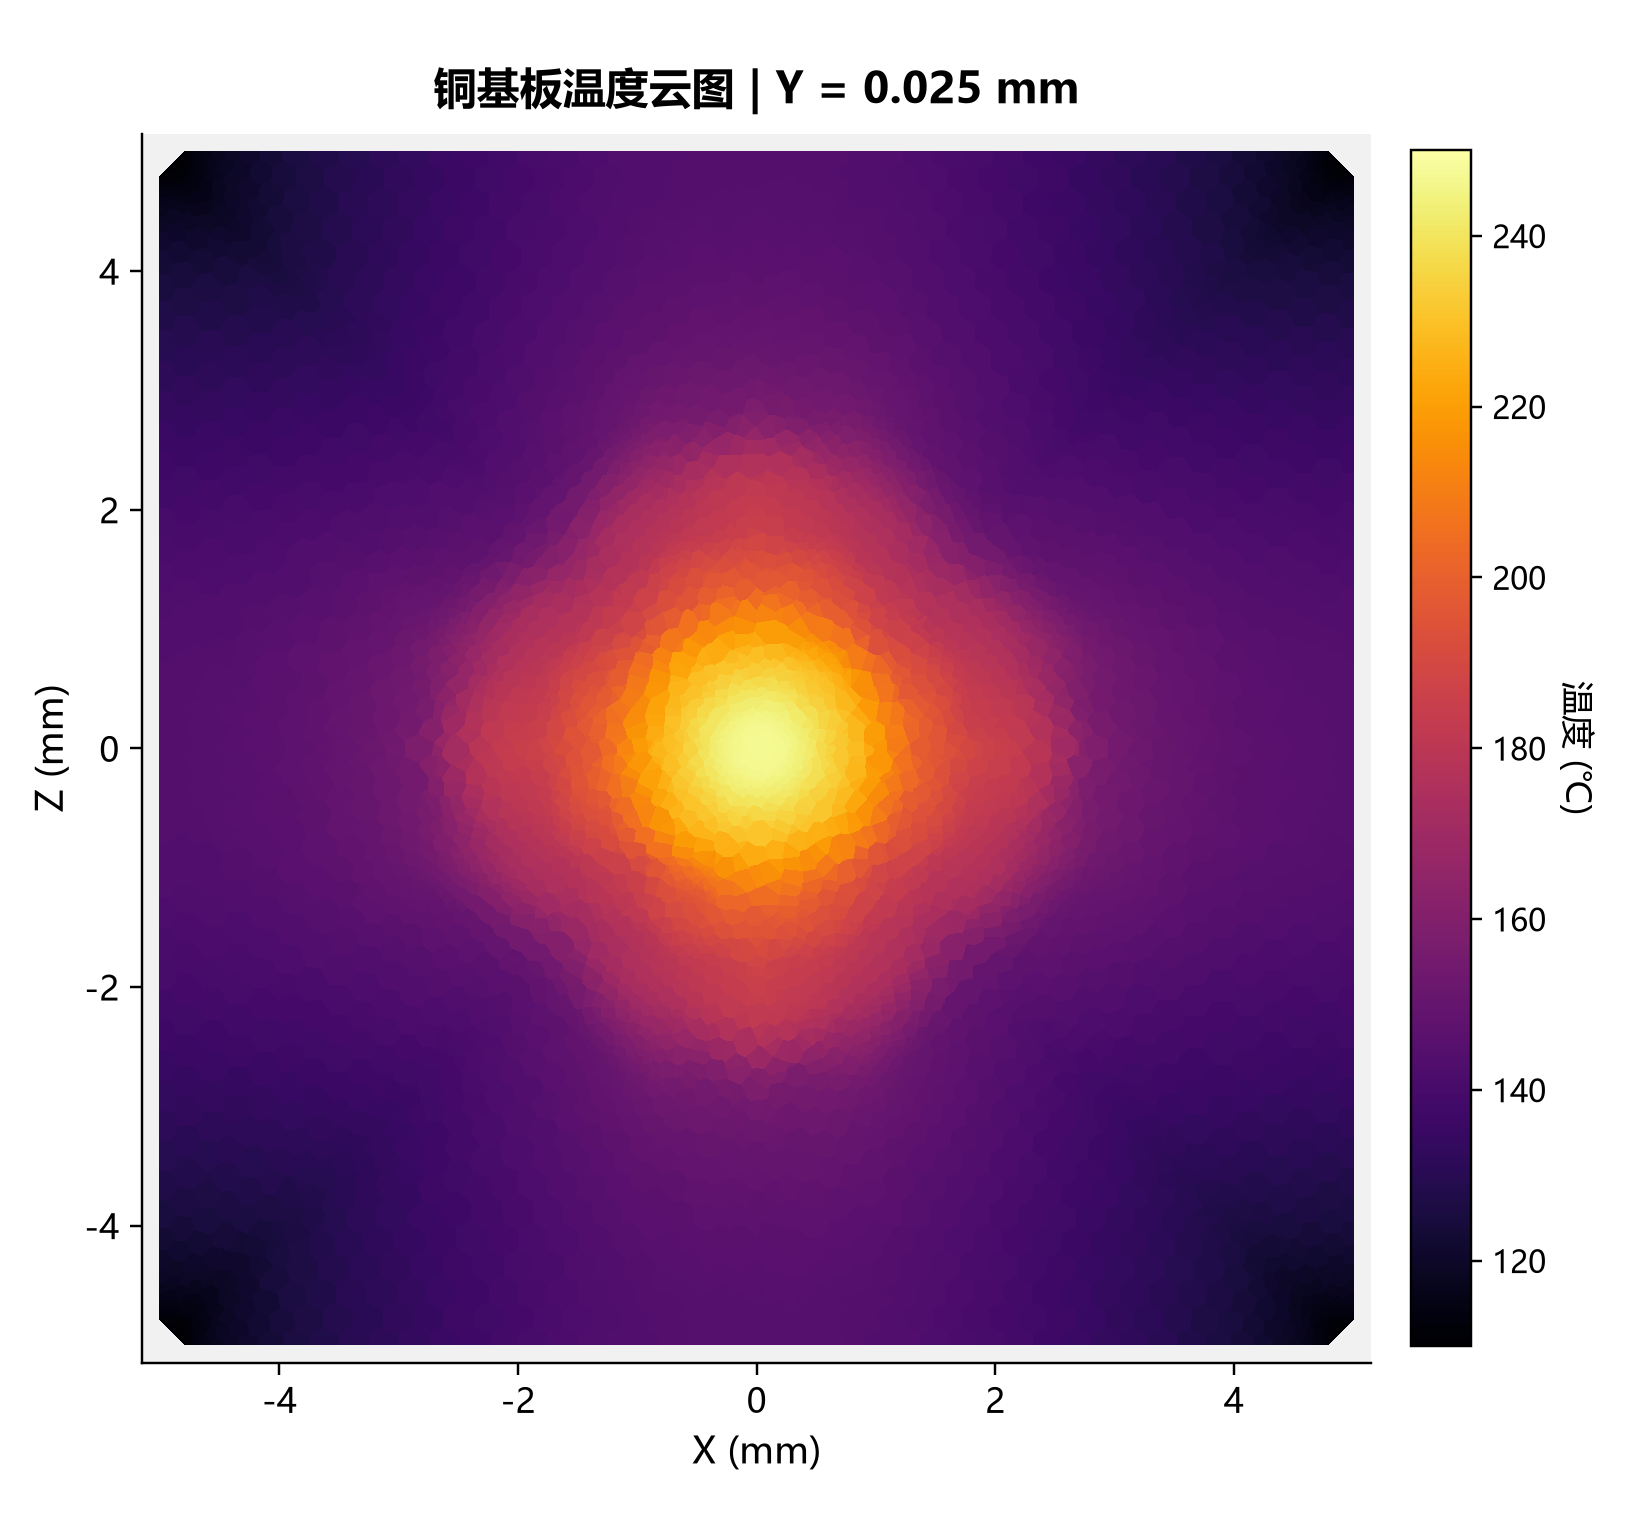
\includegraphics[width=\linewidth]{figs/08_copper_base_temperature.png}
			\caption{六边形微通道铜板温度}
			\label{fig:h5-cu}
		\end{subfigure}
		
		\vspace{4pt}
		
		\begin{subfigure}{0.235\textwidth}
			\centering
			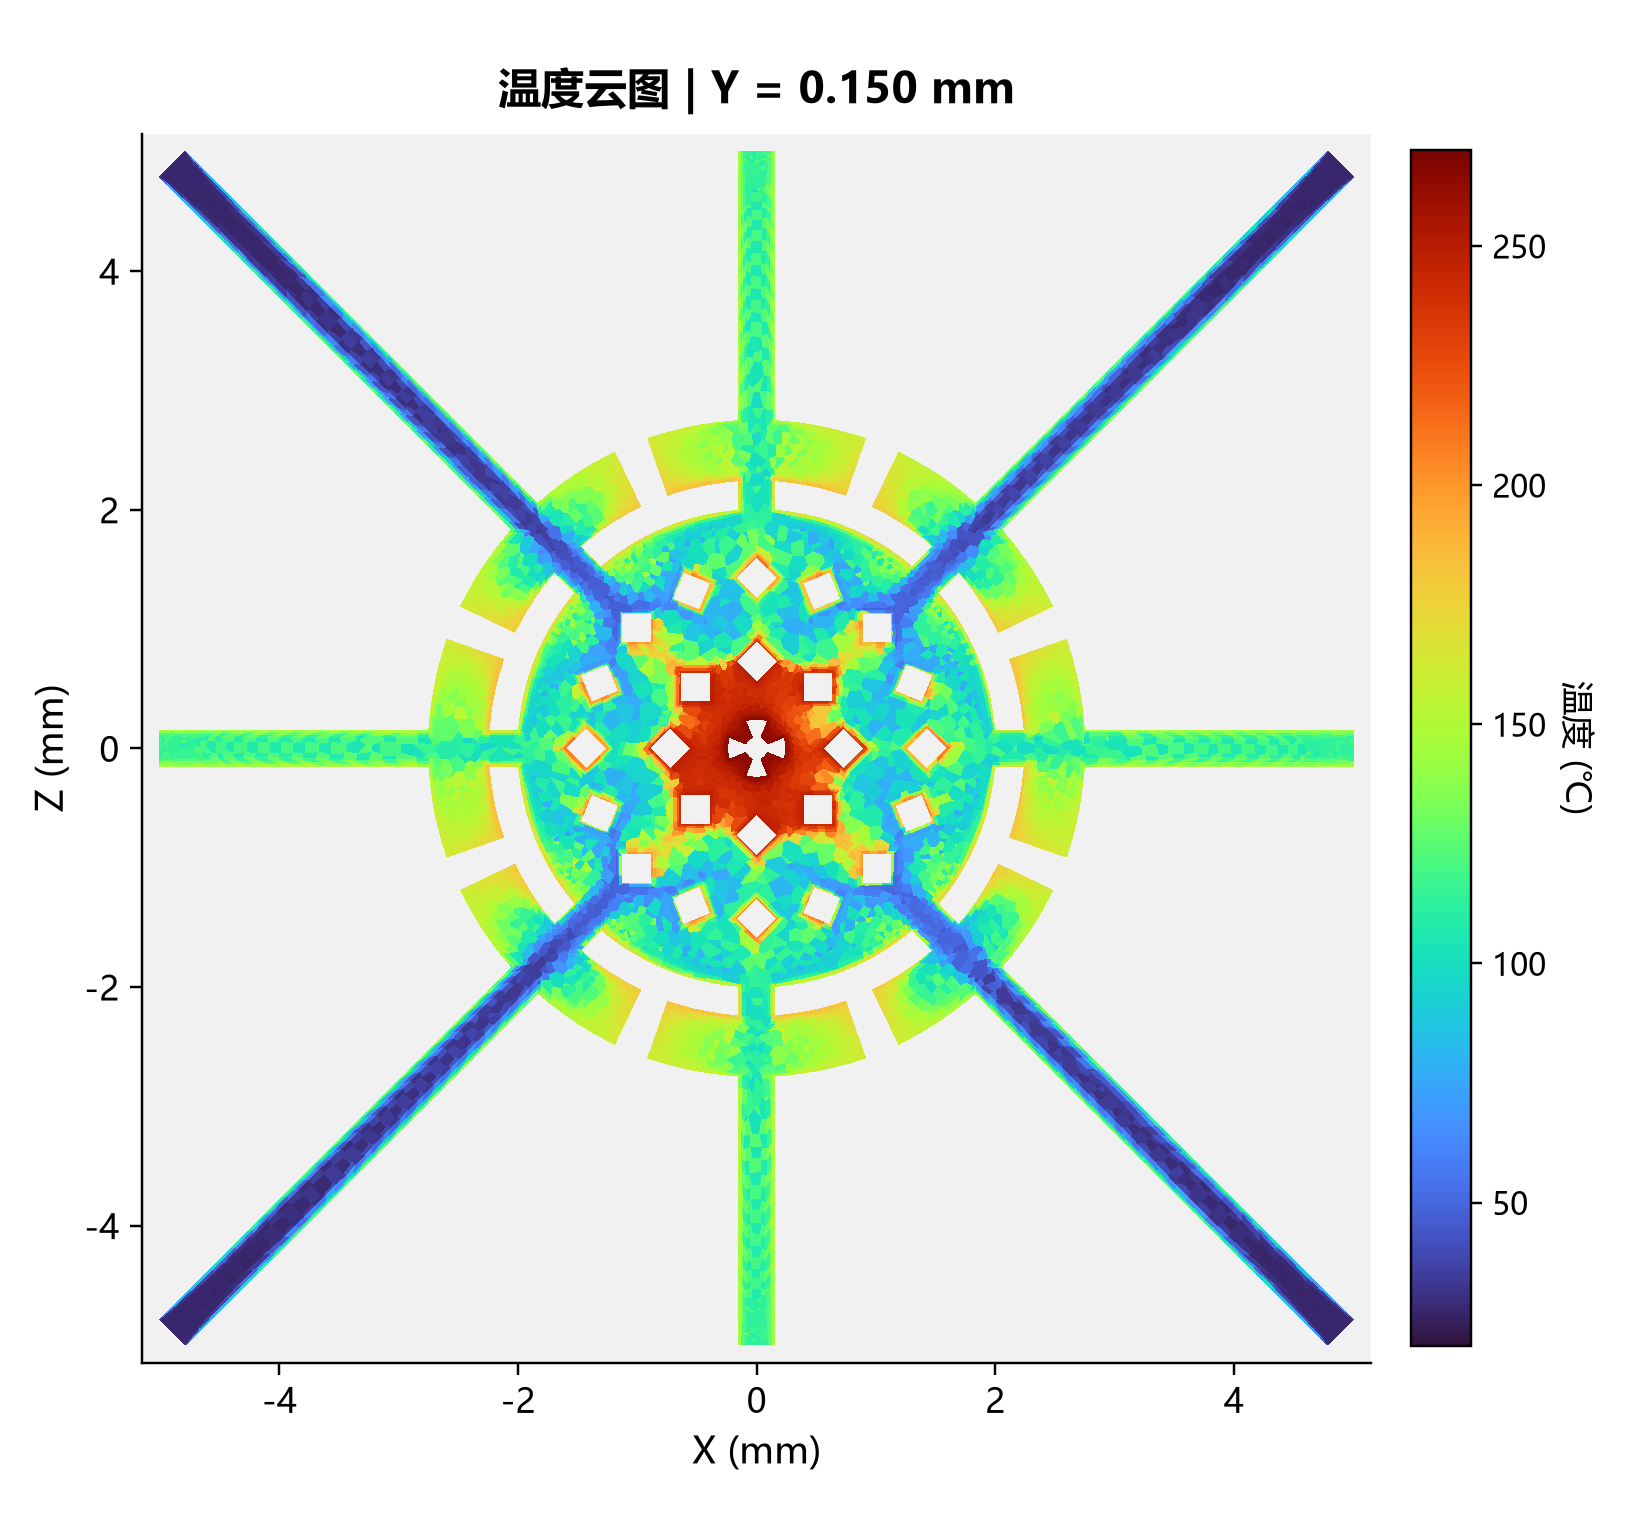
\includegraphics[width=\linewidth]{figs/09_temperature_midplane.png}
			\caption{圆形微通道温度}
			\label{fig:circle-t}
		\end{subfigure}\hfill
		\begin{subfigure}{0.235\textwidth}
			\centering
			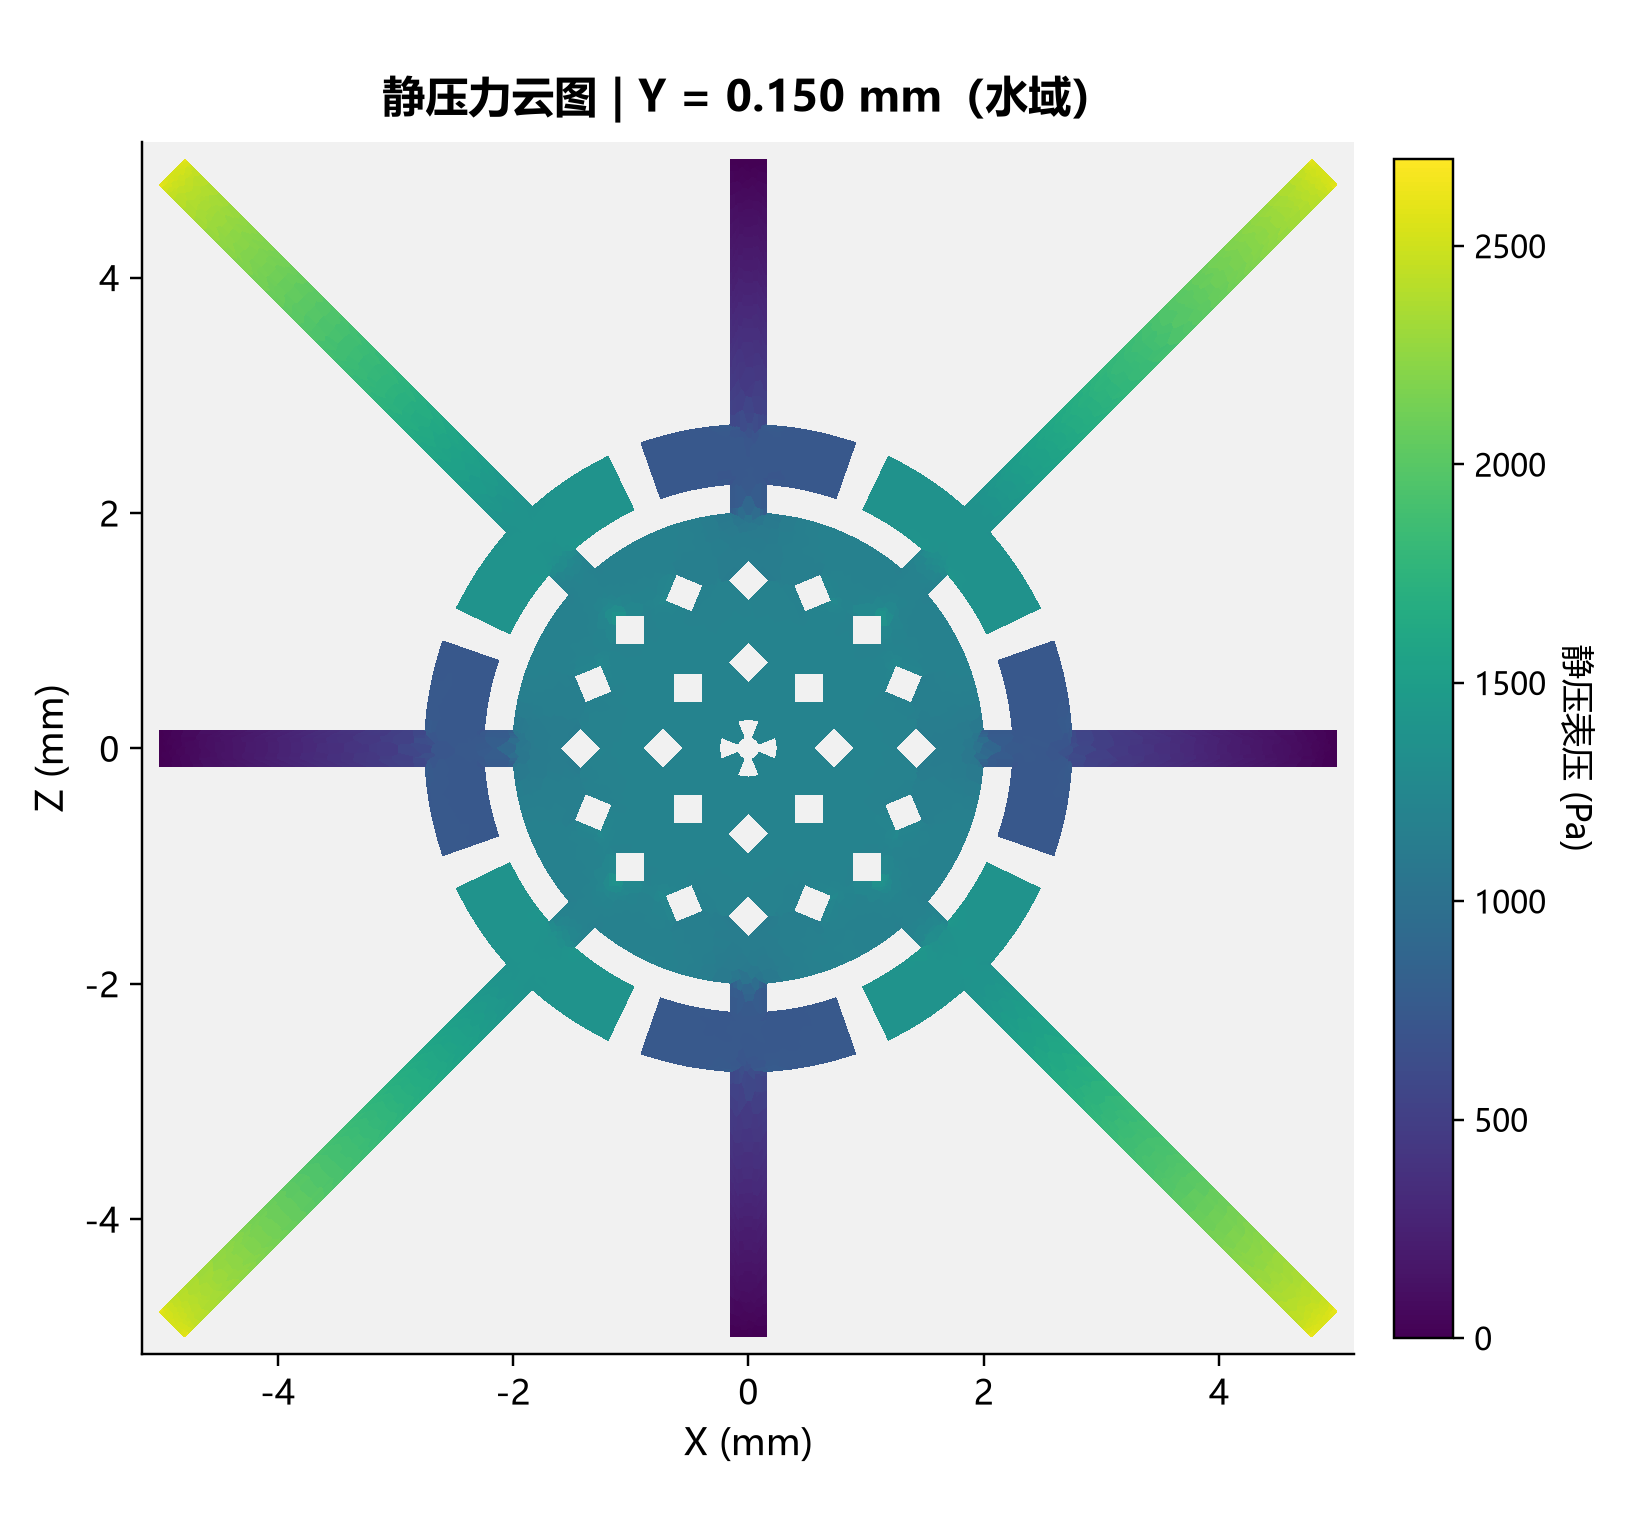
\includegraphics[width=\linewidth]{figs/10_pressure_midplane.png}
			\caption{圆形微通道静压}
			\label{fig:circle-p}
		\end{subfigure}\hfill
		\begin{subfigure}{0.235\textwidth}
			\centering
			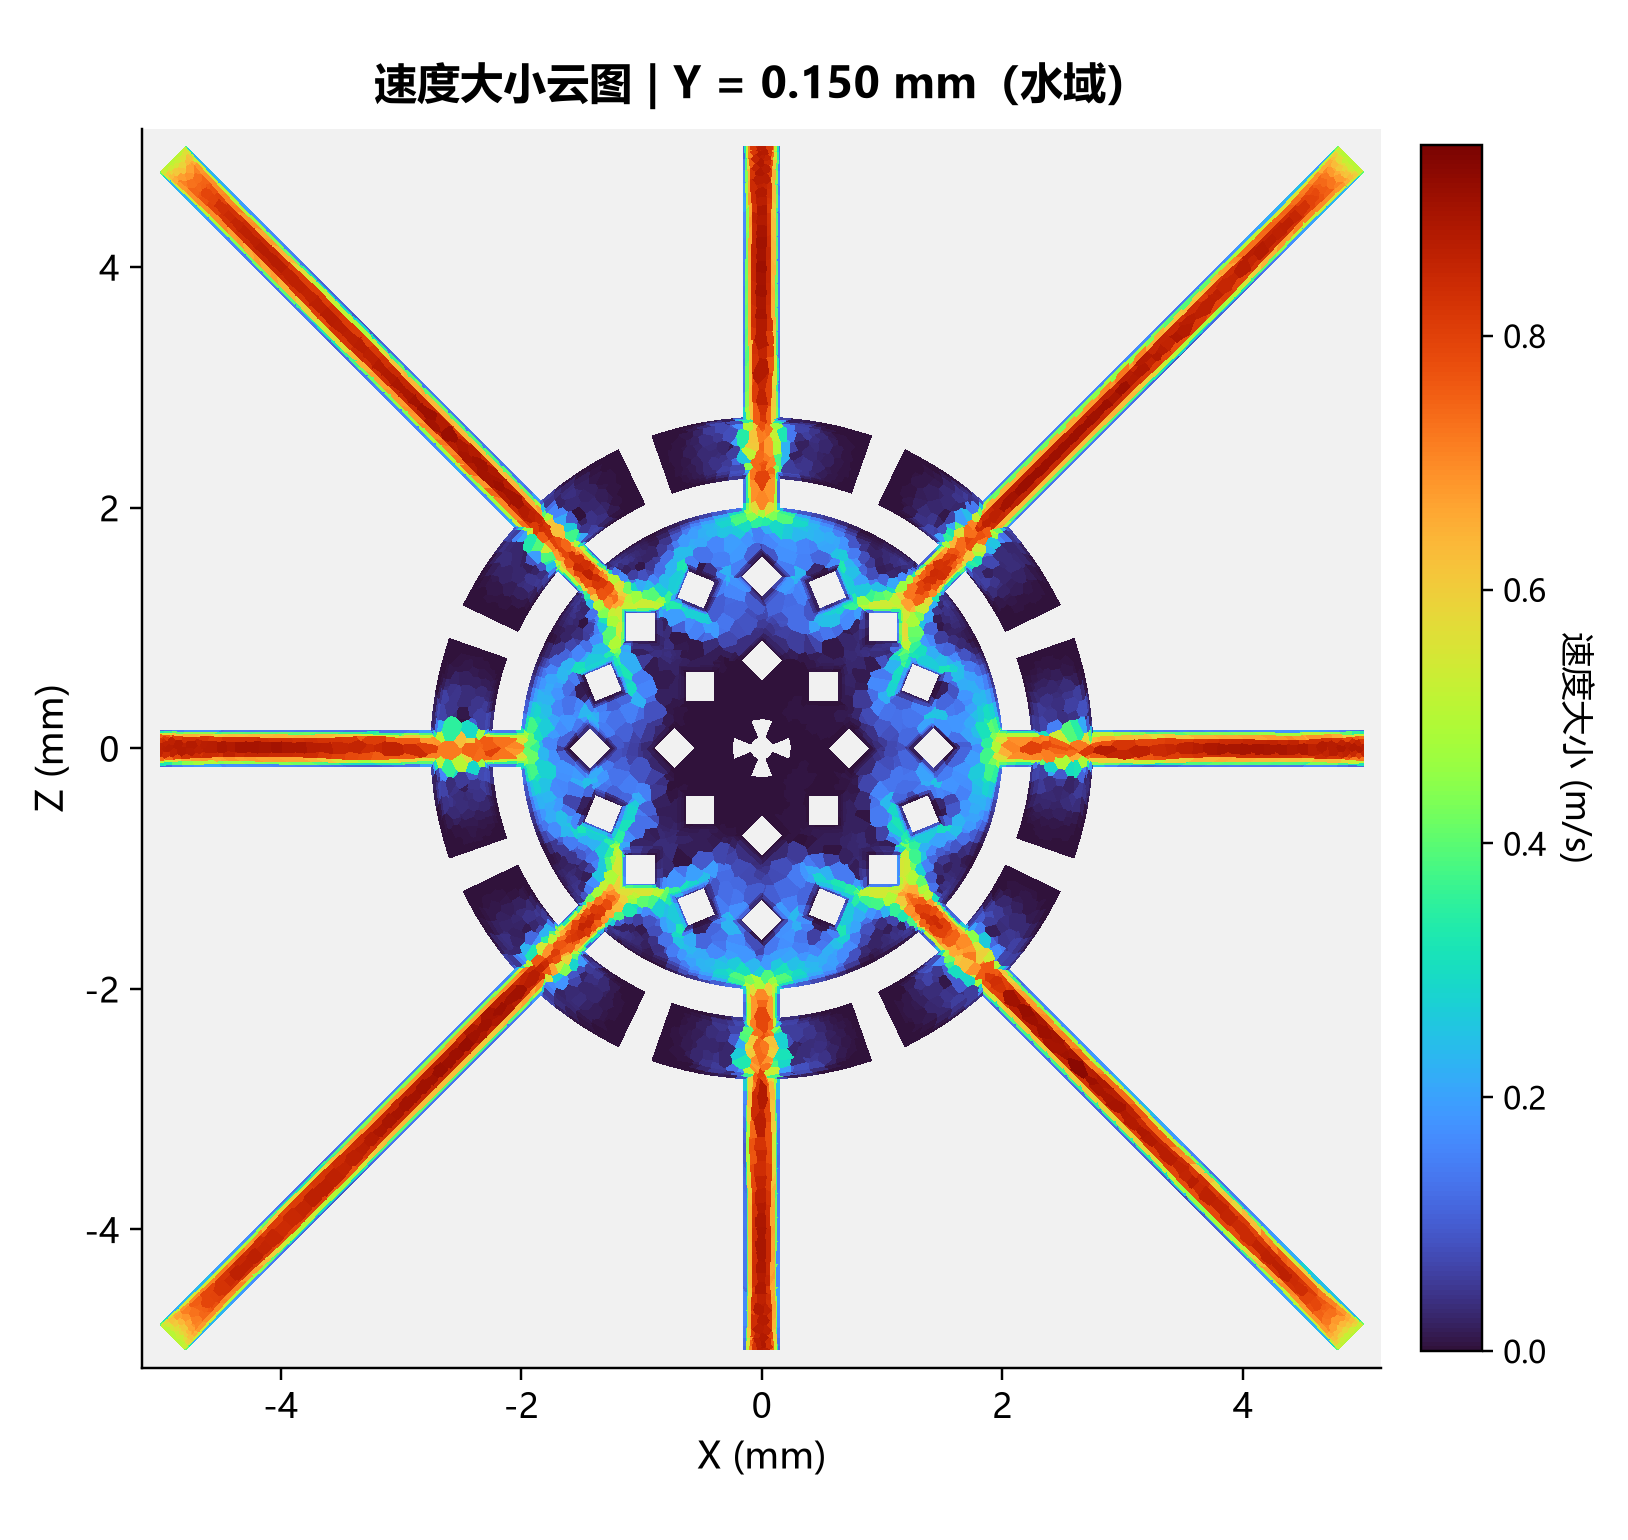
\includegraphics[width=\linewidth]{figs/11_speed_midplane.png}
			\caption{圆形微通道速度大小}
			\label{fig:circle-v}
		\end{subfigure}\hfill
		\begin{subfigure}{0.235\textwidth}
			\centering
			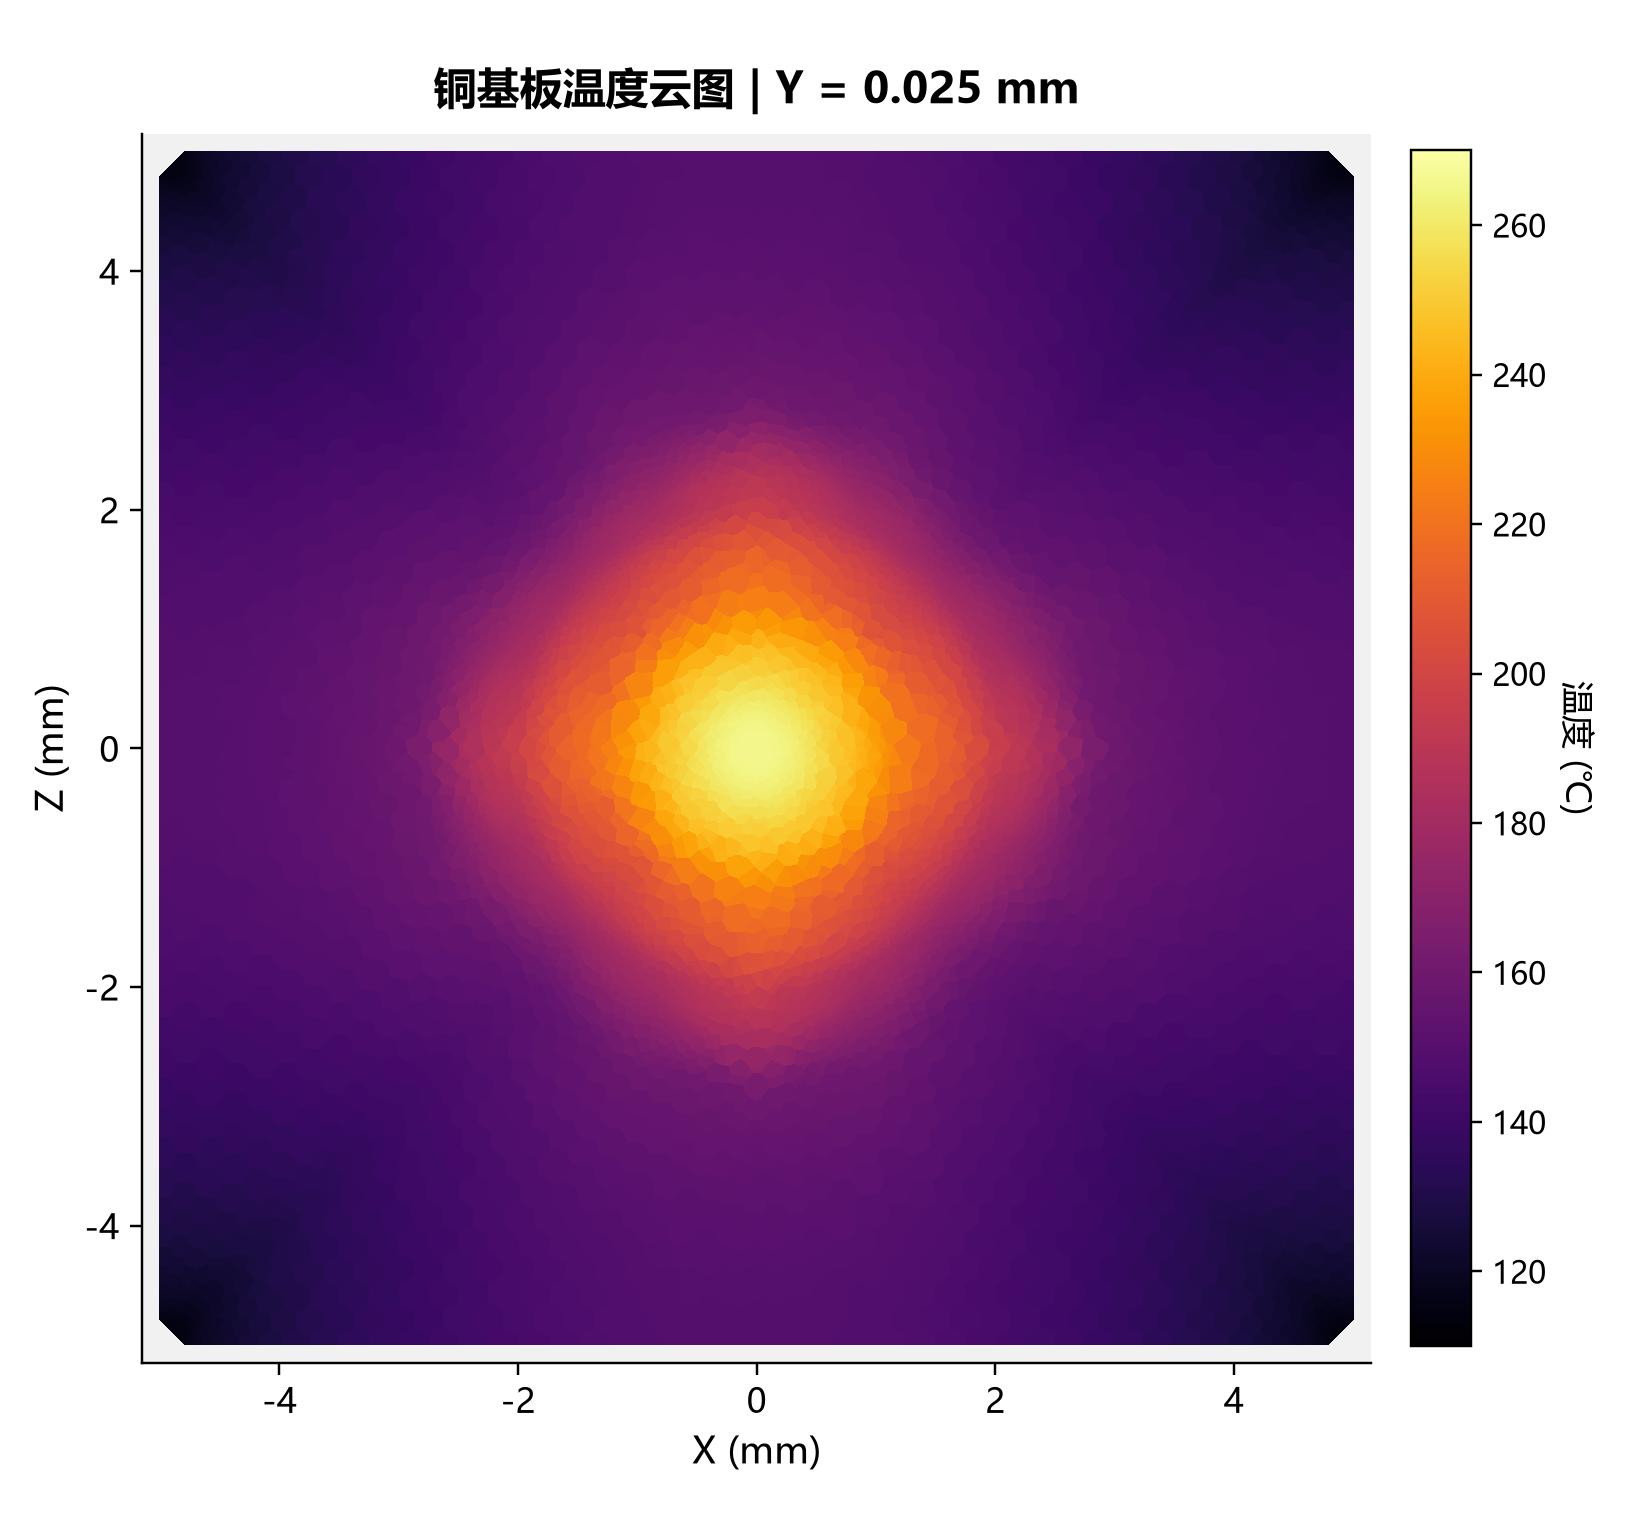
\includegraphics[width=\linewidth]{figs/12_copper_base_temperature.png}
			\caption{圆形微通道铜板温度}
			\label{fig:circle-cu}
		\end{subfigure}
		\caption{复现算例的后处理云图： (a)--(l) 为流道的参考结果。三行均依次为水侧 $Y=0.150$ mm 中截面的温度、静压（表压）与速度大小，以及铜基板 $Y=0.025$ mm 截面的温度。灰白空区为截面外或固体遮罩}
		\label{fig:repro}
	\end{figure}
	
	
	\subsection{复现结果}
	
	\textbf{结构复现}：三种流道的复现已完成，计算结果与论文的趋势一致——
	流量增加时结温总体下降、压降增加；热流密度增加时结温上升。
	
	\begin{table}[H]
		\centering
		\caption{三种流道的复现情况}
		\label{tab:repro}
		\begin{tabularx}{\textwidth}{@{}Y Y Y@{}}
			\toprule
			\rowcolor{ydzjlight} 流道形态 & 复现关注内容 & 结果 \\
			\midrule
			方形微通道 & 方形流路及中心扰动结构的影响 & 已完成，趋势与论文一致 \\
			六边形微通道 & 六边形布局及局部流动组织 & 已完成，趋势与论文一致 \\
			圆形微通道 & 环形流路及流体分配的影响 & 已完成，趋势与论文一致 \\
			
			\bottomrule
		\end{tabularx}
	\end{table}
	
	
	
	\textbf{物性核查}：在 298.15 K 校验点，原水物性函数相对参考值
	\textbf{密度偏低约 60.8\%、比热偏低约 10.5\%、黏度偏低约 26.7\%}。
	
	这是一个\textbf{必须记录的重要发现}：它意味着此前所有基于该物性的
	温度与压差结果都存在系统偏差，结构之间的排序也可能受影响。
	本月据此完成了新物性 UDF 的编写与编译，挂接与复算列入后续月份。
	
	【缺数据：新 UDF 挂接后的物性自检结果】\textcolor{red}{王佳蔚补充新的的说明}
	
	% ==================================================================
	\section{阶段性收获}
	
	\subsection{认知上的变化}
	
	\textbf{一、从「整体冷却」转向「按需分区」。}
	原来倾向于把冷板当作一个整体来强化，认为加密结构总归有利。
	现在认识到：热流密度本身不均匀，均匀强化会在低负荷区造成过度冷却，
	\textbf{冷却资源必须按区域配置}。
	
	\textbf{二、物性不是背景条件，而是结论的前提。}
	复核原物性函数之前，我们默认它是正确的。
	发现偏差后才知道：\textbf{在物性不可信的情况下比较结构，等于在错的基准上排序}。
	因此把「物理性质」放在结构比较之前的做法是必要的。
	
	
	
	% ==================================================================
	\section{下月计划}
	
	\begin{table}[H]
		\centering
		\caption{下月工作计划}
		\label{tab:plan}
		\begin{tabularx}{\textwidth}{@{}Y Y c@{}}
			\toprule
			\rowcolor{ydzjlight} 事项 & 预期产出 & 时间 \\
			\midrule
			挂接新水物性 UDF 并完成物性自检 & 物性校验记录 & 第 1 周 \\
			补齐小块划分图，明确划分依据与数量 & 小块划分方案 & 第 1--2 周 \\
			建立统一的评价指标体系 & 指标定义表 & 第 2--3 周 \\
			小块内的形态与扰流单元仿真 & 形态对比数据 & 第 3--4 周 \\
			完成自控基础学习并形成控制算法提要 & 学习笔记与控制提要 & 第 2--3 周 \\
		\end{tabularx}
	\end{table}
	
	% ==================================================================
	\begin{thebibliography}{99}
	  \bibitem{ao} Ao C, Xu B, Chen Z. Design and performance optimization of novel microchannel heat sinks for high-power electronic chips[J]. International Communications in Heat and Mass Transfer, 2026, 178: 111803.
	  \bibitem{ref1} 隋增光, 林昊晟, 隋云任, 等. 数据中心吸收式节能节水技术研究与应用进展[J]. 制冷学报, 2026, 47(1): 37-50. 
	  \bibitem{ref2} Xu H, Wang Y, Tian W, et al. Thermal performance optimization of dual-bridge arm SiC IGBT modules via microstructure-modified microchannel heat sinks under double-sided liquid cooling[J]. International Communications in Heat and Mass Transfer, 2026, 176: 111339. 
	  
	  
	  \bibitem{ref5} Wang M, Xie J, Bu J, et al. Thermo-hydraulic effects of asymmetric-height and fractal bifurcation channels combined with impingement in microchannel heat sinks[J]. Applied Thermal Engineering, 2026, 298: 130998. 
	  \bibitem{ref6} 张乾坤, 李红艳, 吕碧纯, 等. 叶脉仿生微通道换热器流动与传热特性的数值研究[J]. 制冷学报, 2025, 46(4): 52-60. 
	  
	  \bibitem{ref7} Yang G, Tang Y, Sun Y, et al. Fabrication of microchannel heat sinks using additive manufacturing: A review[J]. Renewable and Sustainable Energy Reviews, 2026, 233: 116879.
	  
	  \bibitem{ref8} Hu Z, Yan W, Wang S. Study on the Thermal Performance of a Specially-Shaped Vapor Chamber for Cooling High Heat Flux Chips[J/OL]. Thermochimica Acta, 2026.
	  

	  \bibitem{ref13} Ansari D, Kim K Y. Hotspot thermal management using a microchannel-pinfin hybrid heat sink[J]. International Journal of Thermal Sciences, 2018, 134: 27-39. 
	  
	  \bibitem{ref15} Ma D, Liu Y, Zhang X, et al. Experimental and numerical investigation of the thermohydraulic performance of a variable-period sinusoidal microchannel heat sink[J]. Applied Thermal Engineering, 2025, 262: 125234. 
	  
	  \bibitem{ref16} 王雅博, 诸凯, 崔卓, 等. 冷却水进出方式对芯片散热器换热性能影响[J]. 机械工程学报, 2018, 54(10): 188-194.
	  
	  \bibitem{ref17} Choi W W, Bang S H, Shin H C, et al. Experimental and numerical study of a high-performance air-cooled N-type manifold microchannel heat sink for large-area applications[J]. International Communications in Heat and Mass Transfer, 2026, 175: 110986.

	 
	  \bibitem{ref20} Indhe M J, Sur A, Yadav A K, et al. Integrating CFD, molecular dynamics, and AI techniques for thermal management of heat transfer devices in microelectronic chip cooling using nano-enhanced PCMs and hybrid cooling systems[J]. International Journal of Thermofluids, 2026, 32: 101587. 
	  \bibitem{ref21} Nie C, Wang H, Li H, et al. Flow and heat transfer characteristics of pin-fin microchannel heat sink with associated diversion structure[J]. International Communications in Heat and Mass Transfer, 2026, 175: 111004.
	  \bibitem{yin} Yin Y, Wang Z, Ma S, et al. A novel coaxial open annular TSV pin-fin embedded in microchannels to comprehensively improve the thermal stability, signal integrity, and heat transfer of 3D integrated circuits[J]. International Communications in Heat and Mass Transfer, 2026, 172: 110619. 
	  \bibitem{seong} Seong H B, Gwon J G, Lee M S, et al. Numerical study and ANN analysis on heat transfer and flow characteristics of microchannel heat sink with inclined rib–pin fin in in-line and staggered arrangements[J]. International Communications in Heat and Mass Transfer, 2026, 178: 111593. 
	  \bibitem{ref24} Lorenzini D, Green C, Sarvey T E, et al. Embedded single phase microfluidic thermal management for non-uniform heating and hotspots using microgaps with variable pin fin clustering[J]. International Journal of Heat and Mass Transfer, 2016, 103: 1359-1370. 
	 
	  \bibitem{yuan} 袁永帅, 等. 当前芯片散热技术方法和特点研讨[J]. 2024.
	  \bibitem{xiong} 熊园园, 等. 基于内嵌式微通道芯片散热结构设计研究综述[J]. 2024.
	  
	  % ---------- 控制方向补充文献（来源：项目计划书 + AI 辅助补充）----------
	  \bibitem{wu} 吴睿康. 电子器件主动液冷散热的建模及实验研究[D]. 杭州: 浙江大学, 2020.
	  \bibitem{ji} 季俊杰. 微通道冷却芯片及其热点的动态特性研究[D]. 杭州: 浙江大学, 2021.
	  \bibitem{laguna} LAGUNA G, VILARRUBI M, IBANEZ M, et al. Numerical parametric study of a hotspot-targeted microfluidic cooling array for microelectronics[J]. Applied Thermal Engineering, 2018, 144: 71-80.
	  \bibitem{tao} TAO F, ZHANG H, ZHANG C. Advancements and challenges of digital twins in industry[J]. Nature Computational Science, 2024, 4(3): 169-177.
	  \bibitem{brunton} BRUNTON S L, KUTZ J N. Data-Driven Science and Engineering: Machine Learning, Dynamical Systems, and Control[M]. 2nd ed. Cambridge: Cambridge University Press, 2022.
	  \bibitem{astrom} ASTROM K J, HAGGLUND T. PID Controllers: Theory, Design, and Tuning[M]. 2nd ed. Research Triangle Park: Instrument Society of America, 1995.
	  \bibitem{vignon} VIGNON C, RABAULT J, VINUESA R. Recent advances in applying deep reinforcement learning for flow control: Perspectives and future directions[J]. Physics of Fluids, 2023, 35(3): 031301.
	  \bibitem{wangy} WANG Y, HE X, HUA Y, et al. Closed-loop forced heat convection control using deep reinforcement learning[J]. International Journal of Heat and Mass Transfer, 2023, 202: 123655.
	  \bibitem{wangyz} WANG Y Z, LI Y B, AUBRY N, et al. Performance analysis of reinforcement learning algorithms on intelligent closed-loop control on fluid flow and convective heat transfer[J]. Physics of Fluids, 2023, 35(7): 077101.
	  \bibitem{mnih} MNIH V, KAVUKCUOGLU K, SILVER D, et al. Human-level control through deep reinforcement learning[J]. Nature, 2015, 518(7540): 529-533.
	\end{thebibliography}
\end{document}
